%
%  LaTeX source:
%  This is a skeleton thesis, provided by (?) Wolfgang Meuck
%  to be copied, along with thesisstyle.sty to your computer.
%
%  Slightly modified by Andrew Kurn, May 2009
%
\documentclass[12pt,letterpaper,oneside]{book}
% Use either 11pt or 12pt! 10pt is too small, although supported. 

\usepackage{epsfig}
\usepackage{multirow}
\usepackage[T1]{fontenc}
\usepackage{array}
\usepackage{booktabs,amsmath}
\usepackage{makecell}
\usepackage{rotating}
\usepackage{multicol}
\usepackage{slashed}
%\usepackage{slashbox}
\usepackage{float}
\usepackage{amsmath}
\usepackage{subfigure}
\usepackage{afterpage}
\usepackage[titletoc]{appendix}

% Load the package
\usepackage[acronym]{glossaries} 
% Generate the glossary
\makeglossaries
\usepackage[xindy]{imakeidx}
\makeindex


\newacronym{QCD}{QCD}{Quantum Chromodynamics}
\newacronym{ATLAS}{ATLAS}{A Torroidal LHC ApparatuS}
\newacronym{LHC}{LHC}{Large Hadron Collider}
\newacronym{CERN}{CERN}{European Organization for Nuclear Research}
\newacronym{LHCb}{LHCb}{LHC-beauty}
\newacronym{CMS}{CMS}{Compact Muon Solenoid}
\newacronym{ALICE}{ALICE}{A Large Ion Collider Experiment}
\newacronym{eV}{eV}{electronvolt}
\newacronym{TRT}{TRT}{Transition Radiation Tracker}
\newacronym{SCT}{SCT}{Semiconductor Tracker}
\newacronym{IBL}{IBL}{Insertable B-Layer}
\newacronym{EM}{EM}{Electromagnetic}
\newacronym{MET}{MET}{Missing Transverse Energy}
\newacronym{JES}{JES}{Jet Energy Scale}
\newacronym{GSC}{GSC}{Global Sequential Calibration}
\newacronym{JVT}{JVT}{Jet Vertex Tagger}
\newacronym{ISR}{ISR}{Initial State Radiation}
\newacronym{FSR}{FSR}{Final State Radiation}

%\newacronym{qcd}{QCD}{Quantum Chromodynamics}



\usepackage[headings]{thesisstyle}
% Options plain and headings are supported. 

% This makes use LaTeX's new font selection scheme (nfss).
\usepackage[T1]{fontenc}

% You might consider using postscript fonts.
% `Times' can be included used this: (2nd line is for math fonts)
\usepackage{times}
\usepackage{mathptm}  
\newcommand{\MET}{\ensuremath E_T^{miss}}
\newcommand{\vMET}{\ensuremath \vec{E}_T^{miss}}
\newcommand{\PT}{\ensuremath p_{\mathrm {T}}}
\newcommand{\vPT}{\ensuremath \vec{p}_{\mathrm {T}}}
% The following packages might be useful for formula typesetting and
% for the inclusion of graphs, respectively.
%\usepackage{amsmath,amssymb}
\usepackage{graphicx}

% Substitute your information 
\author{Arthur James Horton}
\qualifications{BSc., University of Prince Edward Island 2010}
\qualifications{MSc., Simon Fraser University 2013}
\title{THE JET ENERGY SCALE AT ATLAS USING Z+JET EVENTS}
%\approvaltitle{The Jet Energy Scale at ATLAS Using Z+jet Events}
\degree{Master of Science}
\department{Physics \\ Faculty of Science}
\submitdate{Spring 2013}
%\thesistype{thesis}   % standard is "thesis"
\entity{Department}   % standard is "Department"
%\copyrightyear{}      % standard is current

% If you want to grant the copyright instead of reserving it,
% uncomment the next line!
%\grantcopyright   

% Insert here the members of your examining committee 
\chair{Dr. Eldon Emberly (Chair)\\
Associate Professor}
\committee{Dr. Michel Vetterli, Senior Supervisor\\
Professor}
\committee{Dr. Dugan O'Neil, Supervisor\\
Associate Professor}
\committee{Dr. Bernd Stelzer, Supervisor\\
Assistant Professor}
\committee{Dr. Corina Andreoiu, Internal Examiner\\
Assistant Professor\\
Department of Chemistry}

\approvaldate{22 March, 2013}

\abstract{
Jets, collimated sprays of subatomic particles, are an important component of the final state in high-energy proton-proton scattering.  
A correct jet energy scale is therefore essential to the success of the ATLAS experiment.  
In this thesis the missing transverse projection fraction method is used to measure the absolute jet response in Z+jet events where the Z decays into a pair of leptons.  
This measurement complements similar measurements made using $\gamma$+jet events while extending the calibration to lower energies.  
The possibility of taking advantage of the differing fraction of events in each sample with gluon-initiated jets as a method for deriving a parton-dependent jet response is also explored.  
Preliminary results are shown to agree with Monte Carlo predictions within their statistical uncertainty.  
}

% Use this command to compile the chapters individually. This saves
% time when writing.
%\includeonly{chap3}

\begin{document}
\frontmatter          % switches to roman page numbering
\maketitle

%\chapter[Dedication]{}  % writes `Dedication' into table of contents,
			% but not on actual page 
\begin{center}
%\Large
%\emph{\`A tous ceux que j'aime:}
%\\
%\emph{Mum, Dad, Amy, M\'{e}lanie, Justin, Eli, M\'{e}m\`{e}re, P\'{e}p\`{e}re, Ron, et sp\'{e}cialement Ryan.}
\end{center}

% end of dedication

\chapter{Acknowledgments}



% end of acknowledgements

\newpage
\addcontentsline{toc}{chapter}{\contentsname}
\tableofcontents

\newpage 
\addcontentsline{toc}{chapter}{\listtablename}
\listoftables

\newpage
\addcontentsline{toc}{chapter}{\listfigurename}
\listoffigures

\newpage
\addcontentsline{toc}{chapter}{Glossary}
%Print the glossary
\glsaddall
\printglossary[title=Acronyms,nonumberlist]
%[type=\acronymtype,title=Abbreviations]

\mainmatter 
% Here comes the content of your thesis. 
% You should not write the text here, but include each chapter
% separately with the \include command.

%Chapter 1

\chapter{Introduction}

\section{The Standard Model}
\label{SM}
For the last 50 years particle physicists have very successfully described the short distance interactions of elementary particles using the Standard Model.  
The Standard Model consists of two quantum field theories: the Electroweak Theory and \gls{QCD}, which describe the interactions of 12 fundamental spin $\frac{1}{2}$ fermions.  
While the Standard Model contains no explanation for gravity, dark matter, dark energy, etc. it does remain the most successful model available to describe reality on the smallest scales and at the highest energies.  

\begin{table}
  \centering
  \begin{tabular}{ |c|c|c|c|c|c|}
  \hline
   fermion & mass [GeV] & spin & electric charge & colour charge & generation \\
  \hline
  \multicolumn{6}{|c|}{charged leptons} \\
  \hline
    e    & 5.11 x$10^{-4}$ & $\frac{1}{2}$ & -1 & no & 1 \\
  $\mu$  & 1.06 x$10^{-1}$  & $\frac{1}{2}$ & -1 & no & 2 \\
  $\tau$ & 1.78            & $\frac{1}{2}$ & -1 & no & 3 \\
  \hline
  \multicolumn{6}{|c|}{neutral leptons} \\
  \hline
  $\nu_e$      & 0 & $\frac{1}{2}$ & 0 & no & 1 \\
  $\nu_{\mu}$  & 0 & $\frac{1}{2}$ & 0 & no & 2 \\
  $\nu_{\tau}$ & 0 & $\frac{1}{2}$ & 0 & no & 2 \\
  \hline
  \multicolumn{6}{|c|}{up-type quarks} \\
  \hline
  u & 2.3 x$10^{-3}$ & $\frac{1}{2}$ & $+\frac{2}{3}$ & yes & 1 \\ 
  c & 1.28           & $\frac{1}{2}$ & $+\frac{2}{3}$ & yes & 2 \\
  t & 173.5          & $\frac{1}{2}$ & $+\frac{2}{3}$ & yes & 3 \\
  \hline
  \multicolumn{6}{|c|}{down-type quarks} \\
  \hline
  d & 4.8 x$10^{-3}$ & $\frac{1}{2}$ & $-\frac{1}{3}$ & yes & 1 \\
  s & 9.5 x$10^{-2}$ & $\frac{1}{2}$ & $-\frac{1}{3}$ & yes & 2 \\
  b & 4.18           & $\frac{1}{2}$ & $-\frac{1}{3}$ & yes & 3 \\
  \hline
  \end{tabular}
  \caption[Properties of known spin-$\frac{1}{2}$ bosons in the Standard Model.]
        {\small Properties of the known spin-$\frac{1}{2}$ fermions in the Standard Model~\cite{PDG}.  The quark masses have been estimated using the $\overline{\mathrm{MS}}$ renormalization scheme at a scale $\mu = 2$ GeV, and while the neutrino masses are non-zero, they are small enough that they are approximated as zero for the purposes of this thesis.}
\label{table:Fermions}
\end{table}


The fermions, listed in Table~\ref{table:Fermions}, are categorized into three generations of four particles, with each generation being a heavier copy of the previous one.  
Each generation includes two quarks, particles that have colour charge and are therefore subject to the strong force described by \gls{QCD}, and two leptons that have no colour charge.  
The six types (flavours) of quarks are organized into generational pairs, the up (u) and the down (d), the charm (c) and the strange (s), and the top (t) and the bottom (b).  
Similarly each generation of leptons is composed of one charged lepton, known as the electron (e), the muon ($\mathrm{\mu}$), and the tau ($\mathrm{\tau}$), and their neutral counterparts the neutrinos ($\nu_{\mathrm{e}}, \nu_{\mu}, \nu_{\tau}$).  
In addition to each of these matter particles there is a complimentary anti-particle, which has the opposite charge to it's regular counterpart and is denoted using an over bar.  
It is worth noting that the entirety of the periodic table of elements, and therefore all regular matter, require only the first generation of particles to construct.  
The Standard Model also includes spin 1 bosons which mediate the various forces included in the theory (see Table~\ref{table:Bosons}). 

\begin{table}
  \centering
  \begin{tabular}{ |c|c|c|c|c|c|}
  \hline
  interaction     & boson             & mass [GeV] & spin & electric charge &  colour charge \\ \hline
  \multicolumn{6}{|c|}{force carrying bosons} \\ \hline
  electromagnetic & $\gamma$ (photon) & 0          & 1 & 0 & no \\ \hline
  \multirow{2}{*}{Weak} & $W^{\pm}$ & 80.39 & 1 & $\pm1$ & no  \\ 
                        & Z & 91.19 & 1 & 0 & no \\ \hline
  strong & g (gluon) & 0 & 1 & 0 & yes \\ \hline 
  \multicolumn{6}{|c|}{non-force carrying bosons} \\ \hline
  --- & Higgs & 125.09 & 0 & 0 & no \\ \hline
  \end{tabular}
  \caption[Properties of known bosons in the Standard Model.]
        {\small Properties of known bosons in the Standard Model.}
\label{table:Bosons}
\end{table}



The electroweak interaction has four force carrying bosons: the photon, the Z, and W$^{\pm}$.  
As the name suggests, while the electroweak force is unified for at high energies, at lower every day energies the electroweak symmetry is spontaneously broken into the electromagnetic force and the weak force.  
In the Standard Model this breaking is explained by introducing a new scalar field with a non-zero vacuum expectation value, known as the Higgs field.  
This breaking into two separate forces also allows the W and Z bosons to acquire their very large observed mass through the Brout-Englert-Higgs (BEH) mechanism.  
This large mass for the W and Z bosons also leads to the relatively short range of the weak interaction.  
This Higgs field also allows the fermions in the Standard Model to obtain mass as well.  
A measurable consequence of this theory is the presence of a massive spin-0 boson called the Higgs Boson, which was discovered in 2012 at the \gls{LHC}.  

As previously mentioned, \gls{QCD} describes the strong force, which affects particles carrying colour charge much like the electric force affects particles carrying an electric charge.  
Unlike electromagnetism which only has one charge, the electric charge, \gls{QCD} has three colour charges known as red, green, and blue.  
Another notable difference between the two is that while the force mediator of the electric force (the photon) has no electric charge itself, this is not the case for the force carriers of the strong interaction (gluons).  
One important consequence of this difference is that the strength of the strong force does not weaken with increasing distance between the particles in question.  
This difference means that quarks cannot be found as individual particles but come in bound `colour neutral' states, a phenomenon known as confinement.  
While these bound states are colour neutral a much weaker residual force still exists, and while it decreases quite rapidly with distance it is this residual force which is responsible for holding protons and neutrons together in the nuclei of atoms.  

These bound states contain an infinite number of quarks/anti-quark pairs constantly being created and annihilated (called sea quarks) and gluons, but the overall identity and properties of a given bound state are determined by their valence quarks.  
Bound states can have either three valence quarks (or anti-quarks) which are known as the baryons, or a quark/anti-quark pair, called the mesons.  
Baryons and mesons are collectively known as hadrons.  
As hinted at above, familiar examples of these bound states include protons (uud) and neutrons (udd).  
As a result of these complicated bound states the masses of the quarks cannot be measured directly, but must be approximated by measuring the bound states and making certain theoretical assumptions~\footnote{The t quark is the exception, as it decays fast enough that no bound states are formed.}.
 

\section{Experimental Particle Physics}
\label{Sec:Experi}
The Standard Model and all of its predictions can be studied in a variety of settings.  
One category of experiment involves accelerating long-lived particles and bringing them to collision inside of a detector, allowing for the study of the shorter lived particles of the Standard Model that are created in the collisions.  
The particles being accelerated can be both elementary (electrons for example) or composite (like protons), with the different choices affecting the types of collisions that will be observed.  
A relevant example of such a detector/accelerator combination is \gls{ATLAS} at the \gls{LHC}.  

The \gls{LHC} is a machine that straddles the border of Switzerland and France at the \gls{CERN} in Geneva.  
While it can produce heavy ion collisions, it is most known for its ability to produce higher energy proton-proton collisions than any other accelerator facility in the world.   
Bringing protons from rest to within a few meters per second away from the speed of light is a multi-step process, a description of which can be found in the LHC Design Report~\cite{LHCDesignReport} while a summary can be found in section~\ref{Sec:LHC}.  

\gls{ATLAS} is a general purpose detector that has been placed in the LHC accelerator ring to observe collisions along with three other detectors.  
There is another general purpose detector known as \gls{CMS}, in addition to two more specialized detectors called \gls{LHCb} and \gls{ALICE}.  
Detectors like \gls{ATLAS} and \gls{CMS} are designed to be able to accurately measure a wide variety of signals allowing them to more fully explore the collisions provided by the \gls{LHC} to push the Standard Model to its limit and search for potential new physics beyond the Standard Model.  
Details on how this is accomplished in ATLAS will be provided in section~\ref{Sec:ATLAS}.  

As the \gls{LHC} collides protons, and therefore quarks and gluons, the most commonly produced objects in the \gls{ATLAS} detector are collimated sprays of particles called jets.  
Jets are the result of an interplay between a high energy colour charged particle being ejected from a collision and the confinement property of the strong force allowing only colour neutral particles to exist.  
The formation of jets will be discussed in greater detail in Sec.~\ref{jets}.  
With this large abundance of jets they are inevitably a signature for a large number of final states being searched for or studied in ATLAS, with many requiring a very accurate energy and momentum calibration for the jets.  
This thesis presents a technique for measuring the jet energy scale \textit{in-situ} using events where jets are produced along with other well measured objects (photons, electrons and muons).  

\section{Units and Conventions}
 
For the remainder of this thesis it will be worth keeping a few particle physics conventions in mind.  
The most commonly used is the non-SI unit of energy, the \gls{eV}, which is the amount of energy a singly-charged particle gains after being accelerated across a potential of 1 Volt.  
One eV is the equivalent of 1.602$\times 10^{-19}$ Joules.  
Energies relevant to this thesis are typically be much larger than a single eV, so gigaelectronvolt (GeV, $10^9$ eV) and teraelectronvolts  (TeV, $10^{12}$ eV) are more commonly used.  
Traditionally electronvolts are also used to describe mass and momentum.  
This is made possible using another particle physics convention which is to set the speed of light c to be unitless and equal to one, allowing mass to be described in terms of eV/c$^2$ (see tables~\ref{table:Fermions} and \ref{table:Bosons}), and momentum to be referenced in terms of eV/c.  
It is also standard practice to treat h ̄ the same way.


%\chapter{Experimental setup}
\label{Experiment}

\section{The Large Hadron Collider}
\label{Sec:LHC}

\section{The ATLAS Experiment}
\label{Sec:ATLAS}

\subsection{The ATLAS Coordinate System}

\subsection{ATLAS Detector: Overview}

\subsection{ATLAS Hardware: Inner Detector}

\subsection{ATLAS Hardware: Calorimeter}

\subsubsection{Electromagnetic Calorimeter}
\label{EMCalo} 

\subsubsection{Hadronic Calorimeter}
\label{Had}

\subsection{ATLAS Hardware: Muon Spectrometer}

\subsection{Triggers}
\label{Trig}

%\chapter{Physics Object Reconstruction}
\label{Reco}

\section{Electron/Photon}
\label{EMReco}
The reconstruction of electrons and photons with the ATLAS detector involves measurements by both the electromagnetic calorimeter and the inner detector.  
The process begins with a list of clusters found using a sliding window with a size equal to 3 x 5 cells ($\eta$ x $\phi$) in the second layer of the EM calorimeter.  
A modified list of tracks from the inner detector is also used, with tracks containing only hits in the TRT being simply copied over and tracks with silicon hits being refit to account for the potentially large radiative energy loss that electrons can experience during their flight~\cite{ATLAS-CONF-2012-047}.  
Tracks become associated with a cluster if they are close enough (0.05 x 0.05 with Si, 0.35 x 0.02 without) and pass some quality criteria.  
Clusters with tracks are candidates for either electrons or converted photons (single or double track).  

At this stage clusters are expanded to 3 x 7 (5 x 5) in the barrel (endcap).  
Clusters with two tracks without pixel layer hits or no single track with more than 4 Si hits are labeled as photon candidates, while clusters with single tracks with pixel hits are labeled as electron candidates.  
The energy of these larger clusters is used as the input energy of the object for calibration, while the $\eta$ and $\phi$ is taken from the track(s) (if present) or the cluster (with no tracks).  

\section{Muons}
\label{Muons}

Muons are reconstructed using information from both the muon spectrometer and the inner detector.  
Muon reconstruction begins by creating station by station muon track segments which are then fit into a combined track.  
The fit takes into account the magnetic field from the toroid magnets and a detailed description of the material density throughout the detector.  
These spectrometer only muon tracks are then propagated through the calorimeter (again taking the energy the muons will deposit into account) back into the inner detector.  
Here they are are combined with tracks left by the muon in the tracking detector which have been reconstructed using the regular all-purpose track reconstruction algorithm that is used.  

\section{Jets}
\label{jets}

A result of confinement (see Sec.~\ref{SM}) is that single particles with colour charge cannot be observed.  
This does not actually eliminate collision where a large amount of energy is transfered to a single quark or gluon.  
When these types of collision do occur (which they do quite frequently at a p-p collider) what is seen is a large `spray' of hadrons all traveling along roughly the same path that the original single particle was moving.  
This spray of particles is the outcome of two processes.  
First as the charged colour particle moves away from its counterparts the energy stored in the colour field builds until a new particle/anti-particle pair is produced.  
The creation of these new particle pairs along with the gluons which are radiated by the initial/secondary particles is known as the parton shower.  
When the amount of energy per particle drops below the pair creation threshold a second stage known as hadronization takes over, where these secondary coloured particles combine into colour neutral particles.  
Collectively these two stages are known as fragmentation.  

As was mentioned in Sec.~\ref{Had} the interactions between hadrons and detectors tend to lead to wide and deep showers that are subject to large fluctuation.  
The large number of hadrons moving in the same direction combined with this showering profile means that accurately measuring the properties of these sprays in the calorimeter can be quite tricky.  
The strategy that is generally used is two staged.  
First a stage where individual particle candidates are constructed followed by a second stage where these particle candidates are combined into groups of nearby particles into what are known as jets.  
Multiple options are available for each stage.  

ATLAS has previously used calorimeter towers (stacks of cells in the calorimeter) and `TopoTowers' (towers with additional noise suppression) as inputs to jet finding algorithms, but they aren't necessarily a good representation of a single particle.  
Tracks in the inner detector are also used, although using only tracks ignores all neutral particle information obtained by the calorimeter.  
The most commonly used input to jet finding algorithms in ATLAS begin with topological clusters.  
 
\subsection{Topological Clusters}

In the context of high energy physics detectors topological (topo) clustering is an algorithm where individual calorimeter cells are grouped together based on how significant the energy deposited within a given cells is relative to the expected noise.  
Togo clusters have the ability to take on a wide variety of three dimensional shapes, which allows them to include a large fraction of the energy deposited by incoming particles while ignoring much of the noise.  

Topo clustering begins by determining the significance of the energy deposited withing each cell, which is defined as the absolute value of the measured energy divided by the average expected noise for that cell.  
All cells above some predetermined threshold, $t_{\mathrm{seed}}$, are then put into a list proto-clusters.  
At this stage any cell above some second threshold, $t_{\mathrm{neighbor}}$, which are `neighbors' to a proto-cluster are added to that proto-cluster.  
In this case neighbors consist of the eight nearest neighbors and next to nearest neighbors in the same layer of the calorimeter as the cell in question, as well as all cells in adjacent layers which overlap or partially overlap with any of these nine cells.  
This step is repeated until there are no longer any neighbors above $t_{\mathrm{neighbor}}$.  
The final stage of cluster building involves adding a single final layer around each proto-cluster of all neighboring cells above some third threshold, $t_{\mathrm{cell}}$~\cite{1603.02934}.  
The thresholds used in topoclustering are usually reported as $t_{\mathrm{seed}}-t_{\mathrm{neighbor}}-t_{\mathrm{cell}}$, where ATLAS uses a 4-2-0 configuration.  
4-3-0 topo clusters are also used in ATLAS to reconstruct low $p_T$ electrons, but they will not be used in this thesis.   

After all clusters have been fully formed there is an additional stage where clusters are split.  
This begins by looking for local maxima within a given cluster, which are defined as having energy above 500 MeV with at least four neighbours, none of which have a higher energy than the cell in question.  
The clustering is run again only considering cells within the larger cluster, only this time instead of merging sub clusters as they meet the cells have their energy split between sub clusters.  
 
While topo clusters do a relatively good job of representing the visible energy deposited in the detector by a given particle they are not perfect.  
Clustering may leave some visible energy outside of the bounds of a cluster, energy may be deposited in dead material, or the energy may simply be mis measured as the response to EM energy of the ATLAS detector (e) is not equal tot he response of hadronic energy deposits ($h$).  
These are the factors which motivate the second collection of clusters used by ATLAS.  
This second collection of clusters begins with the original (EM scale) clusters and applies a series of cell by cells weights in an attempt to correct these vary problems at the cluster level.  
This calibration step is known as local hadronic cell weighting, or the LC scale.  
The applied corrections depend on moments of the cluster, the depth and density of the cluster is used for EM/Had identification for example, as well as the physical location of the cluster to estimate the energy lost to dead material.  
This calibration is Monte Carlo based.  

\subsection{Jet Finding}

In order for it to be possible to meaningfully compare experimental results and fixed order QCD calculation jet algorithms must behave in a way that follows certain criteria~\cite{Blazey:2000qt}.  
These criteria are infrared and collinear safety, which mean that the reconstruction should be insensitive to soft and collinear radiation, respectively.  
A family of jet finding algorithms that satisfies these criteria and are used within the ATLAS collaboration is the $k_t$ family~\cite{Cacciari:2008gp}.  
More specifically the members of this family that are used are $k_t$ jets, Cambridge/Aachen jets, and the most commonly used member anti-$k_t$.  
Objects which are used as inputs to these algorithms within ATLAS include tracks, truth particles (in Monte Carlo samples), cluster, etc.  

These algorithms all begin by constructing a list of pseudo jets, which consists of four vectors representing all of the inputs at the desired scale.  
Next a `distance' between every pair of jets is calculated, where the distance is defined as:

\begin{equation}
  d_{ij}=min\left(p_{\mathrm T,i}^{2n}, p_{\mathrm T,j}^{2n}\right)\frac{\Delta_{ij}^2}{R^2}, 
\end{equation}

where $\Delta_{ij}$ is difference in rapidity and the difference in $\phi$ of the two pseudo jets summed in quadrature, $R$ is a tunable size parameter.  
$n$ determines the behaviour of the algorithm, with $n$=1,0,-1 being the $k_t$, Cambridge/Aachen, and anti-$k_t$ algorithms respectively.  
Additionally for each pseudo jet a distance to the beam pipe is calculated using:

\begin{equation}
  d_{iB} = p_{\mathrm T,i}^{2n}.
\end{equation}  

The jet building is then performed by finding the smallest distance parameter.  
If if corresponds to a pseudo jet/beam pipe distance that pseudo jet is promoted to being a full jet, while if it is a pseudo jet pair those jets are removed from the list and combined into a new pseudo jet which is added to the list.  
While there exists different combination schemes ($p_T$ weighted, $p_T^2$ weighted) ATLAS uses a simple addition of the four-vectors of the pseudo jets using the FastJet implementation~\cite{Cacciari:2011ma}.

\section{Missing Transverse Energy}

While large multipurpose detectors like ATLAS are great at detecting a large range of particles they do not and cannot measure 100\% of the energy of every particle produced in every collision.  
Some of this missed energy is from particles interacting with the detector and having a response lower than one, sometimes the more interesting energy with is missed comes from particles which do not interact with the detector at all (eg. neutrinos).  
As one can imagine it's not always straightforward to measure how much energy your calorimeter did not detect.  
Thankfully in a p-p collider all of the initial momentum of the collision is along the beam line, with the exception of a small (effectively negligible) amount of transverse momentum within the protons themselves.  
Using the conservation of momentum one can use an imbalance in momentum along any given axis in the transverse plane and interpret the missing energy which would balance the momentum as a measurement in itself.  
This quantity is known as the \gls{MET} or $E_T^{miss}$.  


The MET, like jets, can be build using a number of different inputs at various scales.  
For many analyses in ATLAS the most appropriate MET to use is one where all physics objects are used at their fully calibrated scales.  
This is done by starting with some base collection (EM clusters, LCW clusters, tracks, etc.) then adding physics objects while removing overlapping base objects to avoid double counting.  
The final MET is calculated by taking the negative vector sum of the transverse momentum of the remaining base objects and all physics objects.  
This thesis will be using topo cluster based METs with only photons, electrons, and muons being replaced with the full calibrated objects.  





%\chapter{Jet Energy Scale}
\label{JES}

Recalling from Sec.~\ref{jets} that jets evolve through many different stages throughout their life (see Fig.~\ref{JetLevelsFig}) it becomes clear that to reasonably compare experimental results to theoretical results one must decide on a scale to make the comparison at.  
This is usually done by bringing all results to the `particle jet' scale, making the results detector independent easing cross experiment comparisons.  
This is accomplished by carefully studying the relationship between the particle scale jet energy and the detector scale jet energy, known as the \gls{JES}.   
A successful \gls{JES} accounts for pileup, escaped/invisible energy, algorithm effects, etc.  


\begin{figure}[!ht]
  \begin{center}
    \scalebox{0.40}{
      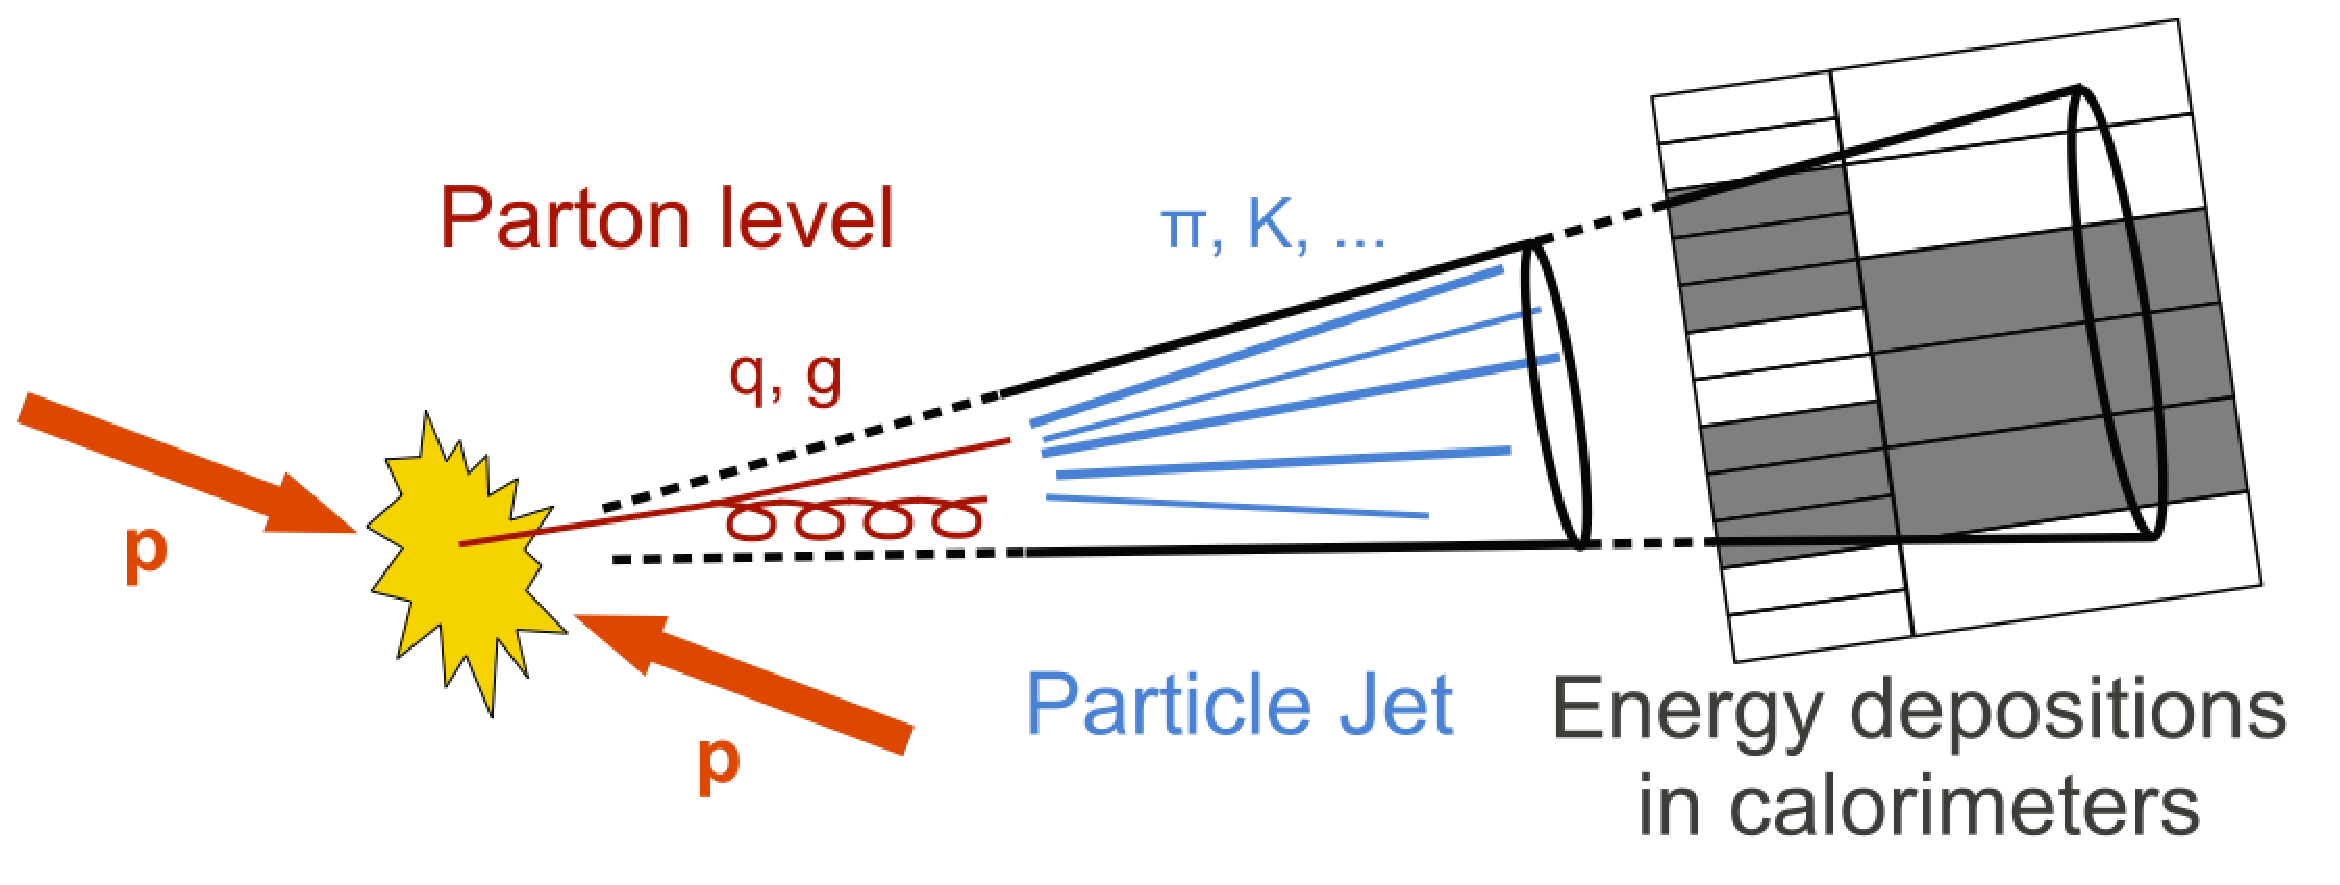
\includegraphics{plots/Chap4/Sketch_PartonParticleCaloJet.eps}
    }
  \end{center}
  \caption[Jet showering evolution.]
      {\small A cartoon outlining the progression from parton level to a calorimeter jet.}
  \label{JetLevelsFig}
\end{figure}

\section{Jet Energy Scale in ATLAS}
\label{ATLASJES}

Calibrating jets withing ATLAS is a multistaged process.  
During the initial jet reconstruction the jet is set to originate from point (0,0,0) in the ATLAS coordinate system, so the first step is to adjust the jet to originate from the reconstructed vertex.  
Next in order to compensate for energy coming from previous collisions and secondary interactions energy is subtracted from the jet, first using the average energy density observe in that given event along with the active area of the jet (calculated using ghost particles~\cite{Soyez:2012hv}) followed by a smaller residual correction.  
With pileup now removed a Monte Carlo based calibration, which completely corrects for the average response as a function of energy and pseudorapidity of jet within that sample, is applied.  

To improve the energy resolution and reduce the flavour dependence of the jets at this stage a series of smaller Monte Carlo calibration are applied.  
These calibrations ideally flatten the dependence of the response on the amount of energy in the first layer of the hadronic calorimeter, the energy in the last layer of the EM calorimeter, the number of charged tracks within the jet, the width of the distribution of those tracks within the jet, and the number of track segments in the muon spectrometer behind the jet.  
These calibrations are collectively known as the \gls{GSC}.  

\begin{figure}[!ht]
  \begin{center}
    \scalebox{0.40}{
      \includegraphics{plots/Chap4/CalibSequence.ps}
    }
  \end{center}
  \caption[Jet showering evolution.]
      {\small A cartoon outlining the progression from parton level to a calorimeter jet.}
  \label{JetCalibSequenceFig}
\end{figure}


The final step involves applying final corrections to account for the observed differences in response between the data which has been collected and the Monte Carlo.  
The response is measured using a series of \textit{in-situ} techniques in both data and Monte Carlo, and the ratio is applied as a final correction to data only.  
In general these \textit{in-situ} techniques make use of a system of physics objects which have been produced back-to-back in $\phi$.  
One object is labeled as the reference object and the response of the second object is measured relative to the reference object.  
These studies can be performed in dijet events where the jets land in different $\eta$ regions (so called eta intercalibration), $\gamma$/Z+jet events where the jet response is measured relative to the boson, and multi jet events where one high energy jet is measured relative to several lower energy jets.  

This study will be using both Z and $\gamma$+jet events to study the jet energy scale in ATLAS.  
Only events where the Z decays into either an electron/positron pair or a muon/anti-muon pair will be considered.  
When it comes to measuring the JES these two types of events are similar and complementary.  
Both offer well measured objects which are ideally produced back-to-back in $\phi$ with a single jet, with a significant difference being that the cross section for $\gamma$+jet is several orders of magnitude larger.   
This larger cross section allows for a larger number of high energy $\gamma$+jet events, stretching out the range which can be calibrated.  
Unfortunately this larger cross section also forces lower energy photon triggers to be prescaled to much lower rates.  
This prescaling at low energy, along with a large number of low energy dijet events being misidentified as $\gamma$+jet events makes Z+jet a much better choice while calibrating the low energy regime.  

\section{Jet Response}

The largest component of the JES is the absolute response, which describes how the calorimeter response to both hadronic and electromagnetic energy deposits within the jet.  
Even for a single incoming hadron there will be some fraction of energy deposited in the calorimeter via EM interactions.  
This is in part because hadrons do have electric charge, but is largely due to hadrons decaying into particles which decay electromagnetically ($\pi^0\rightarrow\gamma\gamma$).  
If we use this division in energy deposit type to write a single particle response, we can say

\begin{equation}
  \label{SingleParticleResponse}
  r(E)=f_{\mathrm{em}}\left(E\right)e+\left[1-f_{\mathrm{em}}\right]\left(E\right)h,
 \end{equation}

\noindent
where $e$ is the response to purely EM energy deposits, $h$ is the response to purely hadronic energy deposits, and $f_{\mathrm{em}}$ is the fraction of the total incoming energy that is deposited electromagnetically.  

This can be further explored by using a simplistic model of a particle showering within a material.  
When a hadron interacts with a nucleus several new hadrons are created, with pions being produced in the largest numbers.  
Thanks to the approximate isospin symmetry of hadronic interactions each flavour of pions is created with equal probability, so if only pions are produced in a given interaction on average 1/3 of these pions will be electromagnetically decaying neutral pions.  
With this model in mind after the first generation of hadrons is produced 1/3 of the available energy is electromagnetic energy deposited by photons resulting from the decay of neutral pions.  
If the charged pions making up the remaining 2/3 of the available energy each have enough energy to cause a subsequent shower, a further 2/9$^{\mathrm{ths}}$ of the energy will be deposited electromagnetically, and so on.  
This dependence of the fraction of EM energy on the total energy of the incident particle can be modeled using

\begin{equation}
  \label{Grooms}
  f_{\mathrm{em}}\left(E\right)=1-\left(\frac{E}{E_0}\right)^{m-1}.
\end{equation} 

\noindent 
Another function which has been used to model the EM fraction with success is 
\begin{equation}
  \label{Wigmans}
  f_{\mathrm{em}}\left(E\right)=a_0+a_1\mathrm{ln}\frac{E}{E_{\mathrm{scale}}}+a_2\left(\mathrm{ln}\frac{E}{E_{\mathrm{scale}}}\right)^2.
\end{equation}

The response of an entire jet can be modeled using
\begin{equation}
  R_{\mathrm{jet}}\left(E\right)=w_hr\left(w_hE\right)+w_ee\left(w_eE\right)
\end{equation}
along with Eq.~\ref{SingleParticleResponse} and either Eq.~\ref{Grooms} or Eq.~\ref{Wigmans}, where $w_h$ and  $w_e$ are the fraction of particles in the jet which will interact hadronically or electromagnetically, respectively.  
These quantities are solely dependent on the parton shower and hadronization processes and are independent of any subsequent showering within the detector.   

\section{$E_{\mathrm T}^{miss}$ Projection Method}
\label{METProj}

The Missing $E_{\mathrm T}$ projecting fraction method is an \textit{in-situ} technique for measuring the jet response.  
It was first developed at the CDF collaboration~\cite{abe1992dijet} to help with their $\eta$ intercalibration, and was later used by the D0 collaboration to extract an absolute jet energy scale~\cite{item/10150/186444}.  
As opposed to the $p_{\mathrm T}$ balance method, which directly compares the measured energy of the jet to the reference object, the MPF measures the response of the entire recoiling system.

The MPF does this using only the measured probe energy and the MET, removing the need to explicitly include the measured jet energy in the response measurement making it independent of the jet algorithm that was used.  
It should be noted that the response still depends on the inputs to the jet finding algorithm, and therefore a MET at the appropriate scale must be used.  
This absence of jet information in the calibration does mean that to perform a full \textit{in-situ} calibration additional algorithm/jet size related corrections do need to be derived.  
This downside can be compensated by the MPF's ability to much more resilient to initial/final state radiation, allowing for looser selection criteria and a relatively larger sample size, as well as its ability to be relatively unaffected by pileup.  

The MPF does take advantage of the balance between the reference object and the recoiling parton to obtain a measure of the true momentum in the recoil, so the derivation of the MPF response begins with 
\begin{equation}
  \label{EQ:MPFPartonLevel}
  \vec{p}_{\mathrm T}^{\mathrm{ref}}+\vec{p}_{\mathrm T}^{\mathrm{recoil}} = 0.  
\end{equation}
\noindent
where $\vec{p}_{\mathrm T}$ is the shorthand for the total momentum of a given particle/object projected into the transverse plane.   
We must also consider this balance at the calorimeter level, which in the simple case of a $2\rightarrow$2 collision can be written as
\begin{equation}
  \label{EQ:MPFCaloLevel}
  R_{\mathrm{ref}}\vec{E}_{mathrm T}^{\mathrm{ref}}+R_{\mathrm{recoil}}\vec{E}_{mathrm T}^{\mathrm{recoil}}=-\vec{E}_{mathrm T}^{\mathrm{miss}},
\end{equation}
\noindent
where we are using $R_{\mathrm{object}}$ to be the response of the calorimeter to that object, and $\vec{E}_{mathrm T}^{\mathrm{object}}$ is known as the transverse energy of the object which is defined as
\begin{equation}
  \vec{E}_{mathrm T}=\frac{E}{\mathrm{cosh}\left(\eta\right)}\hat{p}_{mathrm T}.  
\end{equation}
\noindent
In this thesis only well measured objects are used as references, so $R_{\mathrm{ref}}\simeq1$ and small differences are well known and can be propagated to $\vec{E}_{mathrm T}^{\mathrm{miss}}$.  
By projecting both sides of Eq.~\ref{EQ:MPFCaloLevel} along the directions of the reference object and using Eq.~\ref{EQ:MPFPartonLevel} to remove ${E}_{mathrm T}^{\mathrm{recoil}}$ we obtain
\begin{equation}
  E_{mathrm T}^{\mathrm{ref}}-R_{\mathrm{recoil}}E_{mathrm T}^{\mathrm{ref}}=-\vec{E}_{mathrm T}^{\mathrm{miss}}\cdot\hat{p}_{mathrm T}^{\mathrm{ref}}.
\end{equation} 

\begin{equation}
  \label{EQ:MPFSimple}
  R_{\mathrm{recoil}}=1+\frac{\vec{E}_{mathrm T}^{\mathrm{miss}}\cdot\hat{p}_{mathrm T}^{\mathrm{ref}}}{E_{mathrm T}^{\mathrm{ref}}}.
\end{equation}

This is the MPF that is used to measure the JES \textit{in-situ}.  
What exactly the MPF is doing can be made more clear by expanding out the MET.  
In this ideal case where only the reference object and the recoil exist (using Eq.~\ref{EQ:MPFCaloLevel}) we get that the MPF is just the ratio of the measured energy of the recoil to the measured energy of the reference object.  
In practice the MET will include both initial and final state radiation (ISR and FSR), the underlying event, and pileup.  
This means that the MET can be written as 
\begin{equation}
  \vec{E}_{mathrm T}^{\mathrm{miss}} = -\vec{E}_{T}^{\mathrm{ref}}-\sum_{n}\vec{E}_{mathrm T}^{n},
\end{equation}
where n runs over all energy deposits in the calorimeter that are no related to the reference object.  
Using this definition of the MET we see that the MPF can be written as 
\begin{equation}
  R_{\mathrm{recoil}}=1-\frac{E_{mathrm T}^{\mathrm{ref}}+\hat{p}_{mathrm T}^{\mathrm{ref}}\cdot\sum_{n}\vec{E}_{mathrm T}^{n}}{E_{mathrm T}^{\mathrm{ref}}}=-\frac{\sum_{n}\vec{E}_{mathrm T}^{n}\cdot\hat{p}_{mathrm T}^{\mathrm{ref}}}{E_{mathrm T}^{\mathrm{ref}}}.
\end{equation}
In this form it is much more clear that the MPF is in fact balancing all energy in the event against the reference object.  
Although at first this may seem like a potentially large problem for the MPF to overcome thankfully this is not the case.  
Both the pileup, and to a lesser extent the underlying activity, are uncorrelated with the hard scattering.  
This means that while this extra energy may raise or lower the measured response on an event by event basis when measured over a large sample they will average out to zero (to first order).  

\section{Jet Showering}

The idealized event topology used to derive the MPF ignored the potential effects of a number of subtle issues which have the potential to effect the accuracy of a calibration derived using the MPF.  
One of these effects is the efficiency of the jet reconstruction algorithm being used.  
Jet algorithms are generally good at identifying dense energy deposits in the calorimeter and bunches of high momentum particles are truth level.  
Sadly there is no guarantee that all of the energy in the calorimeter jet came from particles in the particle jet, and likewise there is no guarantee that all of the energy deposited by particles in the truth jet was reconstructed within the calorimeter jet.  
While a $p_{mathrm T}$ balance based calibration would inherently measure and compensate for any potential flow of energy across the boundaries of the jet, an MPF base calibration (being jet algorithm independent) would not.   

While producing Monte Carlo samples within ATLAS the {\sc GEANT4} software toolkit~\cite{GEANT4} is used to propagate particles through the detector and simulate their interactions with the detector material~\cite{Aad:2010ah}.  
These interactions are recorded as `hits', which contain the energy deposited, the position, and time of the deposit.  
A record matching truth particles to all of their resulting hits is also kept.  
These `hits' make it possible to measure the so-called `true response' of a jet in Monte Carlo, which is defined to be the sum of all visible energy deposits in the calorimeter originating from particles within a given truth jet, divided by the energy in that truth jet.  
 





%\chapter{Determining the Jet Energy Scale}
\label{JES2}

\section{Samples}
\label{Sec:Samples}
As seen in Sec.~\ref{ATLASJES} the ATLAS collaboration uses a multistaged approach to calibrate jets, where the final step corrects for any measured response differences observed between selected data and simulated samples.  
The results presented in this thesis are primarily derived using 34.7 fb$^{-1}$ of 13 TeV data taken between April 22nd and October 26th 2016. 
Some results using 3.9 fb$^{-1}$ of 13 TeV data taken between June 3rd and November 3rd 2015 are also presented.  
The measured response in data is compared to results derived using simulated samples.  
In $\gamma$+jet the nominal simulated sample has been generated using the leading order event generator {\sc pythia} 8~\cite{Sjostrand:2007gs} and the NNPDF2.3LO \gls{PDF} set~\cite{Ball:2013hta}.  
The PDF describes how the momentum of the proton is shared between its various parton constituents.  
For the Z+jet nominal sample the hard scattering is simulated as a 2$\rightarrow$3 scattering event using the next-to-leading-order generator {\sc powheg}~\cite{Nason:2004rx, Frixione:2007vw, Alioli:2010xd} and the CTEQ6L1 PDF set~\cite{Pumplin:2002vw}.   
{\sc pythia} 8 provides the fragmentation for both of these samples using $p_{\mathrm T}$-ordered parton showers and the Lund String Model~\cite{ANDERSSON198331}.  
These generated events are propagated through a simulation of the ATLAS detector based on GEANT4~\cite{GEANT4}.  
The interactions of the propagating particles are modeled using the Bertini Cascade model up to 5 GeV, with a smooth transition to the FTFP model for higher energies~\cite{GEANT4Man}.  
In the Bertini Cascade model the incident hadrons enters the target nucleus (modeled as a set of spherical shells) and creates secondary particles based on the free-space cross sections for that collision.  
These secondaries move in straight lines about the nucleus, reflecting or transmitting through the shells and producing secondary and tertiary collisions.  
The cascade ends when all particles, which are kinematically able to, have left the shells.  
The FTFP model simulates the inelastic scattering of hadrons using the FRITIOF model, where one or two QCD strings connect partons in the two nuclei.  
These strings are excited by momentum exchange, and the masses of the strings are chosen randomly.  
These strings then decay into secondary particles using the Precompound model.  
This default ATLAS nuclear interaction model is known as FTFP\_BERT.
 



\section{Event and Physics Object Selection Criteria}
\label{Sec:SelectionCriteria}
\subsection{Reference Selection}
\textit{In-situ} jet calibration techniques require that the jet to be measured is balanced back-to-back with a well measured reference object.  
Criteria are applied to select events with the correct topology, as well as to ensure that the required objects are well measured.  

\subsubsection{Photons}
\label{Sec:Photons}
The first requirement used to select $\gamma$+jet events is that the event must have satisfied a fully efficient single photon trigger.  
In each event that passes this trigger requirement the leading photon (the photon with the highest energy) is considered to be a reference object candidate.  
The photon must be in the central region of the detector ($\mid\eta\mid<$1.37) and have a transverse momentum greater than 25 GeV.  

Each reconstructed photon has a tag associated with it indicating how the photon was reconstructed.  
For this study the tag is required to be either AuthorPhoton or AuthorAmbiguous.  
AuthorPhoton means that no tracks with more than 4 Si hits have been associated with the electromagnetic calorimeter cluster, or that any associated track has no hits in the pixel layers and is associated with a two track vertex in the silicon detector.  
This leads to either unconverted or converted photons, where converted photons refer to photons which have interacted with material in the calorimeter and have been `converted' into an electron/positron pair.  
It should be noted that these converted photons can have one or two tracks associated with them with one track conversions being the result a lost track, with the lost track either being a low energy track which is missed or a high energy track which is on top of the first track.  
AuthorAmbiguous is a tag for all electromagnetic objects (electrons, positrons, photons) that by reconstruction alone cannot be identified as either a photon or an electron.  

In addition to this reconstruction-level identification there is a second, more thorough set of criteria used in this analysis to ensure that the object in question is in fact a photon~\cite{ATL-PHYS-PUB-2016-014}.  
This identification puts requirements on how the energy is distributed within the calorimeter.  
Included are cuts on the fraction of the total energy in the hadronic calorimeter to help eliminate hadrons that fluctuate to have large EM content (through the production of $\pi^0$s), and on the energy in any secondary maximum in the preshower layer to remove neutral pions, which would manifest as two photons in the preshower/calorimeter.  
Differences in the distributions of these shower shape variables have been observed between data and Monte Carlo samples.  
This mismodeling is compensated by applying additional corrections to shower shape variables in the Monte Carlo samples before performing the photon selection.  

To further reduce the number of jets faking photons an additional $p_{\mathrm{T}}$ dependent isolation criterion is applied to the photon, capitalizing on the fact that energy deposits from jets are more diffuse than those from photons.  
This cut requires that the sum of the energy in topo-clusters within a distance $\Delta R=\sqrt{\eta^2+\phi^2}$ = 0.4 of the photon, but excluding the photon itself, must be less than 0.022 $p_{\mathrm{T}}$ + 2.45 GeV.  
There is also a requirement that the sum of the momentum of tracks within $\Delta R$ = 0.2 of the candidate photon, excluding those identified as conversion electrons/photons, is less than 5\% of the momentum of the photon.  
Finally it has been found that the purity of the converted photons can be further enhanced by applying a requirement that the amount of energy of the reconstructed cluster roughly matches the energy of the track.  
In this study, for a two-track converted photon the energy of the cluster divided by the momentum of the track must be between 0.5 and 1.5, with the requirement loosened to be less than 2.0 for single-track converted photons.  


%Author, ID, Pt, eta, isolation, etc.
%Fudge factors for shower shapes in MC
\subsubsection{Z Bosons}
To create a Z boson candidate this study requires exactly two ``good'' leptons which are both the same flavour (electrons or muons) with opposite charge (one particle, one anti-particle). 
These two leptons must reconstruct to have a mass between 66 GeV and 116 GeV, an interval loosely centered around the Z-boson mass (91.19 GeV).  
The requirements for being a ``good'' electron or muon are described below.  

\subsubsection{Electrons}
The trigger used for Z+jet searches for events with two loose (see below) electrons\footnote{In this context ``electron'' refers to both electrons and positrons} with energy above 15 GeV.  
Electrons are required to be within the range of the tracking detectors ($\mid\eta\mid<$2.47) but excluding the transition region between the barrel and the endcap (1.37 $<\mid\eta\mid<$ 1.52).  
A minimum $p_{\mathrm T}$ requirement of 20 GeV is also applied to the electrons.  
In ATLAS, electrons are identified by applying a cut on the output of a multivariate likelihood function, where the inputs are many of the same variables that are used in photon identification~\cite{ATL-PHYS-PUB-2015-041}.  
ATLAS has a number of predefined selection levels (tight, medium, loose, loose+b layer, very loose~\cite{ATL-PHYS-PUB-2015-041}) providing a range of signal acceptance/background rejection levels.  
For this study the loose electron selection criteria are used to maximize statistics.  
Finally there is also an isolation cut applied to electrons, where the loose isolation working point is used.  
This loose working point is set to keep 99\% of all electrons and includes cuts on both the relative energy in the calorimeter and the momentum in the tracker within $\Delta R$ = 0.2 of the electron.  

%not in crack, quality cuts, isolation, etc.

\subsubsection{Muons}
Z$\rightarrow\mu\mu$ events are triggered using the lowest unprescaled dimuon trigger, which required two 10 GeV or 14 GeV muons depending on the data-taking period.   
Muons are required to be within ${\mid\eta\mid<2.4}$ and have a transverse momentum greater than 20 GeV.  
Muons also have predefined identification levels~\cite{ATL-PHYS-PUB-2015-037}; this study uses the loose identification.  
A loose isolation cut is also used for muons, where the isolation area is within $\Delta R$ = 0.2 for the calorimeter and $\Delta R$ = 0.3 for the tracking detector.  

\subsection{Jet Selection}
The jets used in this study are reconstructed with the anti-$k_{\mathrm t}$ algorithm, using 4-2-0 topo-clusters as input at both the EM and LC scale, and with size parameter $R$=0.4.  
As jets are found by searching for large concentrated deposits of energy in the calorimeter, without further conditions imposed, photons and electrons are also expected to appear in the collection of reconstructed jets and must therefore be removed.  
Jets within $\Delta R$ = 0.2 of a photon identified by a separate algorithm (see Sec.~\ref{Sec:Photons}) are not considered, and neither are jets within $\Delta R$ = 0.35 of a lepton.  

Clusters, and therefore jets, can be affected by calorimeter noise bursts, cosmic ray showers, pathological cells in the calorimeter, and other backgrounds.  
The ATLAS collaboration has predefined levels of data cleaning to identify these types of events~\cite{ATLAS-CONF-2015-029}.  
These cleaning levels make use of a pulse quality variable $Q$ which is a quantitative measure of the difference between the measured and expected shape of the electronic signal in the LAr calorimeter cells.  
Both the average of this value for cells within a jet (which is then normalized to the range [0,1]) and the fraction of cells in the jet in the EM/hadronic calorimeter which are 'bad' (defined as $Q$ > 4000) are used in jet cleaning.  
As this study uses MET, any events with a jet above 20 GeV which fail to pass the ``BadLoose'' requirement will be vetoed.  
``BadLoose'' requires that there is not a large amount of negative energy in the jet (no more than 60 GeV resulting from background/noise subtraction), which removes jets strictly from noise.   
It also requires that the most energetic layer of the jet not contain more than 99\% of the total energy of the jet, therefore eliminating electronic noise bursts.   
The normalized measure of the pulse shape quality must be less than 0.8.  
If a significant portion of the jet energy (defined as more than 95\% and 50\% respectively) is in either the EM or hadronic calorimeter most of the energy in that calorimeter must originate from a well described pulse (80\% or 50\% respectively).  
Lastly the total track momentum within a jet is compared to the energy in the calorimeter.  
If the energy in the tracks represents less than 5\% of the total energy in the jet there is likely a large fraction of neutral pions in the jet, so it is required that more than 5\% of the total energy of the jet is collected by the EM calorimeter.  

In 2016 the average number of interactions per bunch crossing in the LHC in a single lumiblock (a period of time of about 1 minute) reached as high as 52.2 (a quantity known as $\mu$)  was achieved on Oct. 14th, 2016.  
With such a high luminosity the possibility for misidentifying a pileup jet as being part of the hard scattering interaction of interest becomes quite high.  
ATLAS uses ghost association of a very large number of artificially added tracks, where the track momentum is set infinitesimally small and jets are reclustered (similar to using ghosts to define area as seen in Sec.~\ref{JES})~\cite{ATLAS-CONF-2013-083}), to match tracks to jets and then uses the vertex information for these tracks and the calibrated jet energy as input to the \gls{JVT}~\cite{ATLAS-CONF-2014-018}.  
The output is a single continuous variable, where 1 corresponds to a perfect match to the primary vertex and 0 corresponds to a pileup jet.  
The recommended JVT cut of 0.59 is used in this study, which corresponds to an average signal efficiency rate of 92\%.  
Events are required to have at least one jet passing this criterion.  
The jet with the largest $p_{\mathrm T}$ is called the leading jet, while the second highest $p_{\mathrm T}$ jet (if it exists) is known as the subleading jet (J2).  

%Well measured jet, JVT

\subsection{Event Topology Requirements}
\label{Sec:EventTopology}
As the goal of this study is to measure the \gls{JES} in the central region of the calorimeter the leading jet is required to have $\mid\eta\mid<$0.8.  
The MPF derivation assumes that the system in question consists solely of the reference object back-to-back with the jet to be calibrated.  
Considering only the selection criteria outlined above this will not always be the case.  
The assumption can be spoiled by any hard radiation emitted by the incoming particles before the hard scattering known as \gls{ISR}, or by radiation emitted by the outgoing parton known as \gls{FSR}.  
These effects can be significantly minimized by explicitly requiring that the leading jet is back-to-back with the reference object in the transverse plane.  
The troublesome topologies can be further removed by requiring that the subleading jet, if present, contains only a small fraction of the total momentum in the system.  
It has been shown in the past that a back-to-back requirement removes almost all of the ISR while the subleading jet requirement removes a large fraction of the FSR~\cite{DougPHD}.  

In this study the back-to-back requirement used is $\Delta \phi \left({\text{leading jet, ref}}\right)>\pi-0.25$.  
The subleading jet, if present, is required to have $p_{\mathrm T}<$ min(12 GeV, 0.3$\times p_{\mathrm T}^{\mathrm {ref}}$) at JES+GSC scale.  
%As previously mentioned these requirements can be looser for an MPF analysis than for a direct balance analysis thanks to the MPF's robustness to ISR/FSR.  


\section{MET Selection}
As mentioned in Sec.~\ref{METProj}, the appropriate MET at the same energy scale as the jets to be calibrated must be used in the MPF method.  
This thesis uses EM and LC scale cluster-based MET to calibrate EM and LC scale jets, respectively.  
In addition to this correct MET scale requirement the MPF derivation presented in this thesis assumes that all reference objects are well measured at the scales used to construct the MET.  
In reality this is not necessarily the case and therefore corrections have been applied to the base MET collections to correct for this fact.  
Electromagnetic objects (electrons, photons) are not perfectly calibrated after reconstruction (despite being reconstructed at EM scale).  
This means that any subsequent calibrations of their energy must be propagated through to the MET.  
As muons are not stopped in the calorimeter a larger correction is needed for them.  
This correction involves removing any potential energy deposits in the calorimeter that have been left by the muons determined by comparing the muon spectrometer and the ID measurements and then adding in the full $p_{\mathrm T}$ of the muon into the MET.  


One additional complication arises for the GSC calibration (explained in Sec.~\ref{ATLASJES}).  
The MPF as presented has no built-in mechanism for testing how well the Monte Carlo simulation models the variables used in the GSC correction.  
A number of methods for incorporating some test of the GSC were explored, including scaling the measured MPF response in each event by the GSC scale factor for the leading jet, propagating the GSC scale factor for the leading jet to the MET before measuring the response, and propagating the GSC scale factor for all jets above 20 GeV through to the MET before making the measurement.  
In the end all three methods agreed well with each other, and showed that the GSC has very little to no effect on the residual MPF calibration measurement.  
The decision was made by the jet/EtMiss group to continue to test the GSC using the second of these methods (propagating the GSC of the leading jet to the MET).  
This correction is used throughout this thesis and the measured response is labeled as either EM+GSC or LC+GSC, depending on the scale of the clusters used to build the MET.  


\section{Measuring the Jet Energy Scale}
\label{Sec:MeasureJES}

\begin{figure}[!ht]
  \begin{center}
  \scalebox{0.6}{
    \includegraphics{plots/Chap5/Data2016_PhotonEMResponseBins/Response_bin_0_25.00.eps}
  }
  \end{center}
  \caption[Example response distribution]
  {\small The distribution of the measured response in ATLAS using $\gamma$+jet events in the 2016 dataset.  The response shown here is at EM scale and for events where the photon has a transverse momentum between 25 and 45 GeV. }
  \label{ExampleRespDist}
\end{figure}


The average response of a jet is a function of the true energy of that jet (see Sec.~\ref{sec:JetResponse}).  
In order to capture this energy dependence the response must be measured in bins of energy or some other quantity that follows energy.  
The steeply falling cross section for both the $\gamma$ and Z+jets processes and the large jet by jet fluctuations in visible energy deposited in the calorimeter would conspire to bias the response high if the most obvious choice was used to simply bin in measured jet energy.  
Instead the $p_{\mathrm T}$ of the reference object is used, which is a sensible choice as it is already being used in the response measurement itself as a measure of the truth jet's $p_{\mathrm T}$.  
To avoid bias from pathological events with very small or unrealistically large response, the MPF response distribution is fit to a Gaussian function rather than taking a simple mean.  
In practice the distribution is fit once with a Gaussian over the full range followed by two additional stages where each subsequent fit is performed within a widow centred on the mean of the previous fit and a width of 1.6 times the sigma of the previous fit.  
An example of the response distribution in the $\gamma$+jet channel at EM scale for photons with transverse momentum between 25 and 45 GeV in the 2016 dataset is shown in Fig.~\ref{ExampleRespDist}.  

\begin{figure}[!ht]
  \begin{center}
  \scalebox{0.6}{
    \includegraphics{plots/Chap5/MappingVsPt_Photon_EM_Data_2016.eps}
  }
  \end{center}
  \caption[Average measured jet momentum Vs. refence $p_{\mathrm T}$]
  {\small The average transverse momentum of the leading jet after the JES and GSC is applied as a function of the energy of the leading photon.  The jets are initially reconstructed using EM scale clusters.  The dotted line is included along the line $p_{\mathrm T}^{\mathrm {ref}}=p_{\mathrm T}^{\mathrm{JES+GSC}}$ to help guide the eye.}
  \label{plot:MappingExample}
\end{figure}


Finally as jets have a predetermined size it is likely that the jet does not contain the full hadronic recoil in the 2$\rightarrow$2 type events used in this study.  
This is especially true at lower energies where jets tend to be wider, and on average $\sim$20\% of the energy is deposited outside of an anti-$k_{\mathrm t}$ R=0.4 jet~\cite{ATLAS-CONF-2015-057}.  
To remove the effect this imperfect match in $p_{\mathrm T}$ has on the binning, the average jet $p_{\mathrm T}$ after the JES and GSC are applied is measured in each bin.  
After the response in each reference $p_{\mathrm T}$ bin is fit and measured the result is then scaled down to the average measured jet $p_{\mathrm T}$ in that bin.  
The average jet $p_{\mathrm T}$ as a function of reference $p_{\mathrm T}$ can be seen in Fig.~\ref{plot:MappingExample}.  

Due to data storage constraints during event reconstruction only jets above a predetermined transverse momentum threshold are kept.  
During the 2015 and 2016 runs at the LHC this threshold for ATLAS was 6 GeV before any calibration.  
For low $p_{\mathrm T}$ V+jet events this threshold has the effect of removing all events where the jet response happened to have fluctuated low.  
This biases the measured response to be higher than it is in reality leading to an unphysical rise in the response at low energies as can be seen in Fig.~\ref{eemumuCompare2016EM} and Fig.~\ref{GammaZCompare2016EM}.  
While this rise is not the result of some detector behaviour it is a feature in the data to be calibrated, and as such is the correct shape of the calibration curve for this dataset.  
This rise in the measured response at low $p_{\mathrm T}$, combined with the higher response in Monte Carlo and the fact that the reconstruction threshold is at the uncalibrated scale, lead to the dip in the relative data/MC response at low $p_{\mathrm T}$ as well.  


\begin{figure}[!ht]
 \begin{center}
  \scalebox{0.6}{
   \includegraphics{plots/Chap5/Photon_IssueFix/mpf_Ratio_EM_2016.eps}
  }
 \end{center}
 \caption[EM scale response using $\gamma$+jet in 2016]
 {\small The EM scale response measured using the MPF technique in $\gamma$+jet events.  Shown in black is the response measured using data from the 2016 dataset, in red is the nominal Monte Carlo sample and in blue is an additional Monte Carlo sample for comparison.  See text for details on the Monte Carlo models.  The lower inset shows the data to Monte Carlo ratio, with the colour of the points corresponding to the simulated sample used in the ratio.  }
 \label{Fig:GammaJetEM2016}
\end{figure}


\begin{figure}[!ht]
  \begin{center}
  \scalebox{0.6}{
    \includegraphics{plots/Chap5/ElectronMuonCompare.eps}
  }
  \end{center}
  \caption[Comparing EM scale response between Z$\rightarrow$ee and Z$\rightarrow\mu\mu$]
  {\small The MPF response as measured using both Z$\rightarrow$ee and Z$\rightarrow\mu\mu$+jet events.  Red points indicate Monte Carlo, black points are data, hollow points are Z$\rightarrow$ee and filled points are Z$\rightarrow\mu\mu$.  Measured at EM+GSC scale using 2016 data.  }
  \label{eemumuCompare2016EM}
\end{figure}

\begin{figure}[!ht]
  \begin{center}
  \scalebox{0.6}{
    \includegraphics{plots/Chap5/PhotonZCompare.eps}
  }
  \end{center}
  \caption[Comparing EM scale response between Z+jet and $\gamma$+jet]
  {\small The MPF response as measured using both Z+jet (with the Z$\rightarrow$ee and Z$\rightarrow\mu\mu$ channels combined) and $\gamma$+jet events.  Red points indicate Monte Carlo, black points are data, hollow points are $\gamma$+jet and filled points are Z+jet.  Measured at EM+GSC scale using 2016 data.   }
  \label{GammaZCompare2016EM}
\end{figure}


\section{Systematic Uncertainties}

While \textit {in-situ} techniques are used to measure the difference in response between data and MC a number of other factors unrelated to the absolute response difference may also affect this measurement.  
These factors include mismodelling of any ISR/FSR, mismodelling of the response of any reference objects, background processes contaminating the measurement in data and so on.  
The potential effect of many of these sources of uncertainty is measured by varying some selection criteria and measuring how these variations affect the central value of the data-to-MC ratio.  
The effects of these individual cut variations are explored in the following sections.  

When using this technique to estimate uncertainties with statistically limited samples one risks inflated systematics caused by statistical fluctuations appearing in multiple measurements.  
Dynamic rebinning of the results is used to reduce the effects of these fluctuations.  
The statistical significance of the shift in the response in a given bin is determined using pseudo-experiments.  
For the nominal response and each variation, N copies of the response are made, where for each event and each copy a weight chosen from a Poisson distribution with a mean of one is applied.  
The bin by bin statistical uncertainty on each variation is then taken as the RMS of the arithmetic means of the nominal/varied ratios of these N copies.  
Bin merging is then done by beginning with the first bin determining if $\left(data/MC\right)_{\mathrm nominal}/\left(data/MC\right)_{\mathrm varied}\neq1$ by more than 1.5 times the statistical uncertainty.  
If this is not true the bin is combined one by one with subsequent bins until this criterion is true, at which point the process moves on to the next bin.  
This procedure is done starting from both the highest and lowest $p_{\mathrm T}$ bin, where in the end the direction yielding the largest number of merged bins is used.  
An example of these pseudo-experiments is shown in Fig.~\ref{ExamplePseudo} while an example of the effect of the entire rebinning process can be seen in Fig.~\ref{Fig:J2GJetEM2016}.  

\begin{figure}[!ht]
  \begin{center}
  \scalebox{0.5}{
    \includegraphics{plots/Chap5/PseudoExperients_GJet_EM_J2down_Data_105-125GeV.eps}
  }
  \end{center}
  \caption[Example pseudo-experiment distribution]
  {\small Distribution of the 100 pseudo-experiments used to estimate the statistical uncertainty on the effect of loosening the subleading jet cut.  This particular distribution is used to determine the uncertainty at EM scale in 2016 data for $\gamma$+jet events with a photon $p_{\mathrm T}$ between 105 and 125 GeV.  }
  \label{ExamplePseudo}
\end{figure}

\begin{figure}[!ht]
  \centering
  \begin{subfigure}{.5\textwidth}
    \centering
    \scalebox{0.4}{
      \includegraphics{plots/Chap5/RadiationPlots_PhotonEM2016/Veto_original.eps}
    }
    \caption{No rebinning}
  \end{subfigure}%
  \begin{subfigure}{.5\textwidth}
    \centering
    \scalebox{0.4}{
      \includegraphics{plots/Chap5/RadiationPlots_PhotonEM2016/Veto_rebinned.eps}
    }
    \caption{With rebinning}
  \end{subfigure}
  \caption{Effect of varying the subleading jet $p_{\mathrm T}$ cut up and down on the EM scale MPF response using $\gamma$+jet events in 2016 before and after rebinning. }
  \label{Fig:J2GJetEM2016}
\end{figure}


\begin{figure}[!ht]
  \centering
  \begin{subfigure}{.5\textwidth}
    \centering
    \scalebox{0.39}{
      \includegraphics{plots/Chap5/RadiationPlots_PhotonEM2016/J2/ResponseVsJ2_45-65.eps}
    }
    \caption{45-65 GeV}
  \end{subfigure}%
  \begin{subfigure}{.5\textwidth}
    \centering
    \scalebox{0.39}{
      \includegraphics{plots/Chap5/RadiationPlots_PhotonEM2016/J2/ResponseVsJ2_400-500.eps}
    }
    \caption{400-500 GeV}
  \end{subfigure}
  \caption[Response as a function of J2 for two $p_{\mathrm{T}}$ bins]
  {\small Response as a function of the fraction of the photon energy contained in the subleading jet (J2) in two different $p_{\mathrm T}$ bins along with the distribution of events plotted against the same variable.  At lower reference $p_{\mathrm T}$ a jet with a small fraction of the reference objects $p_{\mathrm T}$ falls below the reconstruction threshold.  That leads to a large number of events that appear to have no subleading jet.  All selection cuts listed in Sec.~\ref{Sec:SelectionCriteria} have been applied except for the subleading jet cut and the $\Delta\phi$ cut.  }
  \label{Fig:RespVsJ2GJetEM2016}
\end{figure}

\begin{figure}[!ht]
  \centering
  \begin{subfigure}{.5\textwidth}
    \centering
    \scalebox{0.4}{
      \includegraphics{plots/Chap5/RadiationPlots_PhotonEM2016/dPhi/ResponseVsdPhi_45-65.eps}
    }
    \caption{45-65 GeV}
  \end{subfigure}%
  \begin{subfigure}{.5\textwidth}
    \centering
    \scalebox{0.4}{
      \includegraphics{plots/Chap5/RadiationPlots_PhotonEM2016/dPhi/ResponseVsdPhi_400-500.eps}
    }
    \caption{400-500 GeV}
  \end{subfigure}
  \caption[Response as a function of $\Delta\phi$ for two $p_{\mathrm{T}}$ bins]
  {\small Response as a function of the opening angle in azimuth between the reference object and the leading jet ($\Delta\phi$) in two different $p_{\mathrm T}$ bins along with the distribution of events plotted against the same variable.  All selection cuts listed in Sec.~\ref{Sec:SelectionCriteria} have been applied except for the subleading jet cut and the $\Delta\phi$ cut.  }
  \label{Fig:RespVsdPhiGJetEM2016}
\end{figure}

\begin{figure}[!ht]
  \centering
  \begin{subfigure}{.5\textwidth}
    \centering
    \scalebox{0.4}{
      \includegraphics{plots/Chap5/RadiationPlots_PhotonEM2016/dPhi_original.eps}
    }
    \caption{No rebinning}
  \end{subfigure}%
  \begin{subfigure}{.5\textwidth}  \centering
    \scalebox{0.4}{    \includegraphics{plots/Chap5/RadiationPlots_PhotonEM2016/dPhi_rebinned.eps}
  }
  \caption{With rebinning}
  \end{subfigure}
  \caption{Effect of varying the $\Delta\phi$ cut up and down on the EM scale MPF response using $\gamma$+jet events in 2016 before and after rebinning. }
  \label{Fig:dPhiGJetEM2016}
\end{figure}

\subsection{Initial- and Final-state Radiation}
As mentioned in Sec.~\ref{Sec:EventTopology} cuts restricting the maximum transverse momentum of any secondary jets and the opening angle between the jet and the reference object are very good at reducing the effects of FSR and ISR.
However the amount by which these requirements suppress additional radiation is not guaranteed to be well modeled.
Any radiation mismodelling has the possibility of affecting the relative response between data and Monte Carlo, and this effect is measured by varying the associated selection cuts.  
Studies have been preformed in the past which have determines that these cuts essentially are independent and their associated systematics should be treated as such~\cite{ATLAS-CONF-2011-031}.  

\subsubsection{Variation of the Sub-leading Jet Cut}
The subleading jet $p_{\mathrm T}$ cut affects mostly to remove FSR.
This cut is varied from the nominal value ($p_{\mathrm T}<$ min(12 GeV, 0.3$\times p_{\mathrm T}^{\mathrm {ref}}$)) to both a looser value of $p_{\mathrm T}<$ min(12 GeV, 0.4$\times p_{\mathrm T}^{\mathrm {ref}}$) and a tighter one of $p_{\mathrm T}<$ min(10 GeV, 0.2$\times p_{\mathrm T}^{\mathrm {ref}}$).
The effect of this cut variation on the ratio of the measured response in data and MC is found to be quite small (less than half of a percent) as can be seen in Fig.~\ref{Fig:J2GJetEM2016}.
Further insight into the effects of varying the amount of FSR allowed by the selection criteria can be gained by observing how well the MC models the response in data as a function 
of the ratio of the energy in the subleading jet to the energy in the reference object.
As seen in Fig.~\ref{Fig:RespVsJ2GJetEM2016} the absolute value of the measured response does in fact vary as a function of the energy in the subleading jet.
However, this effect is well modeled by the Monte Carlo, with the data/MC response ratio varying only by a percent or so between events with no subleading jets and events with subleading jets containing 45\% of the energy of the photon.
This percent level effect is suppressed because the rest of the selection criteria even without the subleading jet or the $\Delta\phi$ cuts favour a 2$\rightarrow$2 event topology, causing the majority of events to have a soft subleading jet if one exists at all.


\subsubsection{Variation of the Delta Phi Cut}
The $\Delta\phi$ cut affects mostly to remove ISR.  
Just like the subleading jet case, this cut is varied from its nominal value ($\Delta \phi \left({\text{leading jet, ref}}\right)>\pi-0.25$) to both a looser ($\Delta\phi>\pi-0.35$) and a tighter ($\Delta\phi>\pi-0.15$) requirement.
Once again insight can be gained into the effects of this variation by measuring the response as a function of $\Delta\phi$ and observing how well the MC models this behaviour (see Fig.\ref{Fig:RespVsdPhiGJetEM2016}).  

The MPF has a smaller but still present dependence on the $\Delta\phi$ cut compared to the subleading jet cut.  
This dependence is well modeled for events where $\Delta\phi>\pi-0.15$.  
As mentioned in the context of the subleading jet cut simply requiring a ``good'' photon and a jet in the event tends to force them to be back-to-back, even without any explicit cuts forcing this configuration.  
This can be seen in Fig.~\ref{Fig:RespVsdPhiGJetEM2016}, where even without applying any cuts to J2 or $\Delta\phi$ a large number of events have $\Delta\phi>\pi-0.15$.  
This is especially true at higher $p_{\mathrm T}^{\gamma}$, reducing the importance of the $\Delta\phi$ cut and therefore the impact of the cut variation as seen in Fig.~\ref{Fig:dPhiGJetEM2016}.  

\subsection{Uncertainties Related to the Reference Object}
With \textit{in-situ} jet calibration techniques making use of a well measured reference object to estimate the energy of the particle jet it is easy to see how strongly the quality of the calibration depends on the accuracy of the reference calibration.  
Any mismodeling of the energy of the reference object(s) will therefore directly affect the measured MPF.  
This section first describes both scale and resolution uncertainties associated with electromagnetically interacting objects (both electrons and photons).  
This is followed by a description of these uncertainties for the muons used in the (Z$\rightarrow\mu\mu$)+jet channel.  
\subsubsection{E/Gamma Energy Scale and Resolution}

Beginning at the EM scale does not guarantee that EM objects will be properly calibrated after reconstruction.  
It also does not guarantee that the distribution of the energy deposited in the calorimeter will be well modeled in simulated samples.  
As is the case for jets, the ATLAS collaboration uses a number of different steps to fully calibrate both electrons and photons.  
These calibrations include a simulation based multivariate regression that corrects for both energy missed by the reconstruction as well as accounting for where the energy was deposited in the calorimeter~\cite{ATL-PHYS-PUB-2016-015}.  
Also included is an \textit{in-situ} based calibration that corrects for the difference in response between data and simulation.  
This is derived using the known mass peak of the Z in Z$\rightarrow$ee decays.  

The uncertainties from these corrections are propagated through to the jet calibration by measuring the effect of varying the correction up and down by one sigma.  
The effect of this variation is shown in Fig.~\ref{Fig:EGScaleGJetEM2016} for $\gamma$+jet events, and is found to be approximately 1\% over the full $p_{\mathrm T}$ range considered.  
This is much smaller when using Z+jet events.  
This is due to a combination of the uncertainties for electrons being smaller than for photons, the electrons being produced back-to-back cancelling a portion of the scale variations, and because in events where the Z decays into a pair of muons the variation has no effect (see Fig.~\ref{Fig:EGScaleZJetEM2016}).

In addition to the calibration factors used to bring both electrons and photons back to their truth level energy, the electron/photon performance group also measures the energy resolution.  
These studies have shown that the resolution is better in the simulation than it is for data.  
To account for this discrepancy a Gaussian smearing factor is applied to the energy in the simulated pseudo-data.  
The uncertainty on the relative difference in resolution is propagated to the measured JES by varying this smearing up and down by one sigma.  
The effect of this smearing on the EM+GSC response as measured in $\gamma$+jet is shown in Fig.~\ref{Fig:EGResolutionGJetEM2016}.  

\begin{figure}[!ht]
  \centering
  \begin{subfigure}{.5\textwidth}
    \centering
    \scalebox{0.40}{
      \includegraphics{plots/Chap5/EgammaScaleResolution_GJet/EG_SCALE_ALL_original.eps}
    }
    \caption{No rebinning}
  \end{subfigure}%
  \begin{subfigure}{.5\textwidth}  \centering
    \scalebox{0.40}{    
      \includegraphics{plots/Chap5/EgammaScaleResolution_GJet/EG_SCALE_ALL_rebinned.eps}
    }
    \caption{With rebinning}
  \end{subfigure}
  \caption{Effect of varying the photon energy scale up and down on the EM+GSC scale MPF response using $\gamma$+jet events in 2016 before and after rebinning. }
  \label{Fig:EGScaleGJetEM2016}
\end{figure}

\begin{figure}[!ht]
  \centering
  \begin{subfigure}{.5\textwidth}
    \centering
    \scalebox{0.40}{
      \includegraphics{plots/Chap5/EgammaScaleResolution_ZJet/EG_SCALE_ALL_original.eps}
    }
    \caption{No rebinning}
  \end{subfigure}%
  \begin{subfigure}{.5\textwidth}  \centering
    \scalebox{0.40}{
      \includegraphics{plots/Chap5/EgammaScaleResolution_ZJet/EG_SCALE_ALL_rebinned.eps}
    }
    \caption{With rebinning}
  \end{subfigure}
  \caption{Effect of varying the electron energy scale up and down on the EM+GSC scale MPF response using Z+jet events in 2016 before and after rebinning.  Note that the y-axis scale is different from Fig.~\ref{Fig:EGScaleGJetEM2016}. } 
  \label{Fig:EGScaleZJetEM2016}
\end{figure}


\begin{figure}[!ht]
  \centering
  \begin{subfigure}{.5\textwidth}
    \centering
    \scalebox{0.4}{
      \includegraphics{plots/Chap5/EgammaScaleResolution_GJet/EG_RESOLUTION_ALL_original.eps}
    }
    \caption{No rebinning}
  \end{subfigure}%
  \begin{subfigure}{.5\textwidth}  \centering
    \scalebox{0.4}{    
      \includegraphics{plots/Chap5/EgammaScaleResolution_GJet/EG_RESOLUTION_ALL_rebinned.eps}
    }
    \caption{With rebinning}
  \end{subfigure}
  \caption{Effect of varying the photon energy smearing up and down on the EM+GSC scale MPF response using $\gamma$+jet events in 2016 before and after rebinning. }
  \label{Fig:EGResolutionGJetEM2016}
\end{figure}

\Needspace{5\baselineskip}
\subsubsection{Muon Scale and Resolution}
As for electrons and photons, the energy of muons is smeared to improve the agreement between the measured resolution in data and Monte Carlo.  
Muons also have uncertainties associated with both the momentum scale and the smearing applied to the momentum in MC samples~\cite{Aad:2016jkr}.  
The momentum smearing is done independently for both the inner detector and the muon spectrometer.  
The impact of each of these three variations on the ratio of the MPF in data and Monte Carlo is at most on the order of 0.1\% over the full $p_{\mathrm T}$ range measured, with the exception of one large fluctuation in the lowest $p_{\mathrm T}$ bin for the muon spectrometer smearing (see Figs.~\ref{Fig:MuonsScaleZJetEM2016}, \ref{Fig:MuonsIDZJetEM2016}, and~\ref{Fig:MuonsMSZJetEM2016}).  


%\subsection{JVT}

%The effect of misidentifying pileup jets as part of the hard scattering is measured by varying the JVT requirement from its nominal value of 0.59 to both a more restrictive (0.91) and a less restrictive (0.11) value.  
%These values have average signal acceptance rates of 85\% and 97\%, respectively.  
%The choice of a JVT working point has very little effect on the data/Monte Carlo agreement for the MPF, changing by less than 0.02\% over most of the $p_{\mathrm T}$ range considered.  
%This illustrates the relative immunity of the MPF technique to pileup in general.  
%There is a small potential effect at low $p_{\mathrm T}$ where the numerous low energy pileup jets could have a larger effect, but even in this region the agreement never changes by more than a third of a percent.  


\begin{figure}[!ht]
  \centering
  \begin{subfigure}{.5\textwidth}
    \centering
    \scalebox{0.40}{
      \includegraphics{plots/Chap5/EgammaScaleResolution_ZJet/MUONS_SCALE_original.eps}
    }
    \caption{No rebinning}
  \end{subfigure}%
  \begin{subfigure}{.5\textwidth}  \centering
    \scalebox{0.4}{
      \includegraphics{plots/Chap5/EgammaScaleResolution_ZJet/MUONS_SCALE_rebinned.eps}
    }
    \caption{With rebinning}
  \end{subfigure}
  \caption{Effect of varying the muon momentum scale up and down on the EM+GSC scale MPF response using Z+jet events in 2016 before and after rebinning. }
  \label{Fig:MuonsScaleZJetEM2016}
\end{figure}

\begin{figure}[!ht]
  \centering
  \begin{subfigure}{.5\textwidth}
    \centering
    \scalebox{0.4}{
      \includegraphics{plots/Chap5/EgammaScaleResolution_ZJet/MUONS_ID_original.eps}
    }
    \caption{No rebinning}
  \end{subfigure}%
  \begin{subfigure}{.5\textwidth}  \centering
    \scalebox{0.4}{
      \includegraphics{plots/Chap5/EgammaScaleResolution_ZJet/MUONS_ID_rebinned.eps}
    }
    \caption{With rebinning}
  \end{subfigure}
  \caption{Effect of varying the momentum smearing in the ID up and down on the EM+GSC scale MPF response using Z+jet events in 2016 before and after rebinning. }
  \label{Fig:MuonsIDZJetEM2016}
\end{figure}

\begin{figure}[!ht]
  \centering
  \begin{subfigure}{.5\textwidth}
    \centering
    \scalebox{0.4}{
      \includegraphics{plots/Chap5/EgammaScaleResolution_ZJet/MUONS_MS_original.eps}
    }
    \caption{No rebinning}
  \end{subfigure}%
  \begin{subfigure}{.5\textwidth}  \centering
    \scalebox{0.4}{
      \includegraphics{plots/Chap5/EgammaScaleResolution_ZJet/MUONS_MS_rebinned.eps}
    }
    \caption{With rebinning}
  \end{subfigure}
  \caption{Effect of varying the momentum smearing in the MS up and down on the EM+GSC scale MPF response using Z+jet events in 2016 before and after rebinning. }
  \label{Fig:MuonsMSZJetEM2016}
\end{figure}

\subsection{JVT}

The effect of misidentifying pileup jets as part of the hard scattering is measured by varying the JVT requirement from its nominal value of 0.59 to both a more restrictive (0.91) and a less restrictive (0.11) value.
These values have average signal acceptance rates of 85\% and 97\%, respectively.
The choice of a JVT working point has very little effect on the data/Monte Carlo agreement for the MPF, changing by less than 0.02\% over most of the $p_{\mathrm T}$ range considered.
This illustrates the relative immunity of the MPF technique to pileup in general.
There is a small potential effect at low $p_{\mathrm T}$ where the numerous low energy pileup jets could have a larger effect, but even in this region the agreement never changes by more than a third of a percent.


\begin{figure}[!ht]
  \centering
  \begin{subfigure}{.5\textwidth}
    \centering
    \scalebox{0.4}{
      \includegraphics{plots/Chap5/GJet_Systs_EM/JVT_original.eps}
    }
    \caption{No rebinning}
  \end{subfigure}%
  \begin{subfigure}{.5\textwidth}  \centering
    \scalebox{0.4}{
      \includegraphics{plots/Chap5/GJet_Systs_EM/JVT_rebinned.eps}
    }
    \caption{With rebinning}
  \end{subfigure}
  \caption{Effect of varying the JVT requirement to be more/less strict in rejecting pileup jets on the EM+GSC scale MPF response using $\gamma$+jet events in 2016 before and after rebinning. }
  \label{Fig:GJetJVTEM2016}
\end{figure}

\begin{figure}[!ht]
  \centering
  \begin{subfigure}{.5\textwidth}
    \centering
    \scalebox{0.35}{
      \includegraphics{plots/Chap5/Pileup/Photon/EM/ResponseVsMU_45-65.eps}
    }
    \caption{45-65 GeV}
  \end{subfigure}%
  \begin{subfigure}{.5\textwidth}
    \centering
    \scalebox{0.35}{
      \includegraphics{plots/Chap5/Pileup/Photon/EM/ResponseVsMU_400-500.eps}
    }
    \caption{400-500 GeV}
  \end{subfigure}
  \caption[Response as a function of $\mu$ for two $p_{\mathrm{T}}$ bins]
  {\small Response as a function of the average number of collisions per bunch crossing for a given lumiblock ($\mu$) in two different $p_{\mathrm T}$ bins.  This quantity is a measure of both the amount of in time and out of time pileup present in the event.  } 
  \label{Fig:RespVsMUGJetEM2016}
\end{figure}

\begin{figure}[!ht]
  \centering
  \begin{subfigure}{.5\textwidth}
    \centering
    \scalebox{0.35}{
      \includegraphics{plots/Chap5/Pileup/Photon/EM/ResponseVsNPV_45-65.eps}
    }
    \caption{45-65 GeV}
  \end{subfigure}%
  \begin{subfigure}{.5\textwidth}
    \centering
    \scalebox{0.35}{
      \includegraphics{plots/Chap5/Pileup/Photon/EM/ResponseVsNPV_400-500.eps}
    }
    \caption{400-500 GeV}
  \end{subfigure}
  \caption[Response as a function of npv for two $p_{\mathrm{T}}$ bins]
  {\small Response as a function of the number of reconstructed primary vertices in the event (npv) in two different $p_{\mathrm T}$ bins.  This quantity is used as a measure of the amount of in time pileup present in the event.  }
  \label{Fig:RespVsNPVJetEM2016}
\end{figure}


\subsection{Photon Purity}
\label{Sec:purity}
In Sec.~\ref{sec:JetResponse} a simplified model of jet calorimeter showering was presented where after each interaction new pions are created, and on average 1/3 of the pions are $\pi^0$'s which rapidly decay into a photon pair.  
While it is true that on average each pion flavour is produced in roughly equal proportions, this is not necessarily true for any given jet.  
From time to time a jet will fluctuate to have a very large number of neutral pions at some early stage of its development, either during the parton shower or its interaction with the material of the calorimeter, leading to a dense deposit of EM energy.  
This is exactly what the photon/electron reconstruction algorithms look for, and removing this jet is the reason for the strict identification requirements.  
Even with all of the strict identification criteria described earlier in this chapter, the sheer number of dijet events compared to $\gamma$+jet events means that a non negligible number of dijet events will be misidentified as $\gamma$+jet events.  
The misidentified reference jets in dijet events have a lower response than photons, meaning these events will lead to a higher jet response being derived than in true $\gamma$+jet events (the denominator in Eq.~\ref{EQ:MPFSimple} is too small).  
An uncertainty is added to the $\gamma$+jet response measurement to account for this.  

The size of this effect, and therefore the size of the uncertainty that should be assigned to cover it, depends on how large the jet contamination of the photon sample is.  
The purity of the photon sample must therefore be quantified.  
To estimate the background (dijet fakes where one jet fakes a photon) that  satisfies the selection criteria used in this study, sideband regions, which are dominated by dijet fakes, are used.  
Two cuts are chosen which ideally have a large impact on the signal acceptance while at the same time the probability of a background event passing or failing one of these cuts must be independent of whether it passes the other cut.  
In this study the relative energy/momentum isolation cut and the photon identification cut are used (see Fig.~\ref{ABCD}).  

\begin{figure}[!ht]
\begin{center}
\scalebox{0.6}{
  \includegraphics{plots/Chap5/Purity/IsEMIsolCone_25_to_45_GeV_ditributions.eps}
}
\end{center}
\caption[Sideband method]
{\small Diagram showing the signal region and sidebands that are used in the photon signal purity measurement.  LNT is ``Loose-Not-Tight''.  }
\label{ABCD}
\end{figure}

Unfortunately the photon ID cut does have an impact on the fraction of background events that pass the isolation cut.  
In order to resolve this issue a looser photon ID selection criterion is applied before beginning the process.  
This means that in this section events that fail the tight criteria will have passed a loose one, and these events will be labelled as ``loose-not-tight'', or LNT.  

The events that pass both of these cuts are located in region $A$, which has both signal and background events.
Events that fail both cuts fall into region $D$, with regions $B$ and $C$ corresponding to events that pass one cut and fail the other (see Fig.~\ref{ABCD}) .   
Using this labeling and the fact that the background distribution is independent of these cuts, the following equations hold
\begin{equation}
 \frac{A_{\mathrm{data}}^{\mathrm{background}}}{B_{\mathrm{data}}^{\mathrm{background}}} = \frac{C_{\mathrm{data}}^{\mathrm{background}}}{D_{\mathrm{data}}^{\mathrm{background}}},
\end{equation}

\begin{equation}
 A_{\mathrm{data}}^{\mathrm{background}} =  \frac{C_{\mathrm{data}}^{\mathrm{background}}B_{\mathrm {data}}^{\mathrm{background}}}{D_{\mathrm {data}}^{\mathrm{background}}}. 
\end{equation}
\noindent 
Now if regions $B$, $C$, and $D$ are assumed to contain only background events, then $X_{\mathrm{data}}^{\mathrm{background}}=X_{\mathrm{data}}$ for $X=$ $B$, $C$, and $D$, and:

\begin{equation}
 \label{eq:PureSimple}
 \mathrm{Purity} = \frac{A_{\mathrm{data}}^{\mathrm{signal}}}{A_{\mathrm{data}}} = 1-\frac{A_{\mathrm{data}}^{\mathrm{background}}}{A_{\mathrm{data}}} =1- \frac{C_{\mathrm{data}}B_{\mathrm{data}}}{D_{\mathrm {data}}A_{\mathrm {data}}}
\end{equation}
\noindent

This very simple derivation assumes that regions $B$, $C$, and $D$ contain only background, which is not necessarily true.  
This ``signal leakage'' is accounted using a signal only MC sample and measuring the amount of signal in each background region relative to the amount in the signal region.  
That is to say for each region $X$ a correction $\lambda_X\equiv\frac{X_{\mathrm{signal}}^{\mathrm{MC}}}{A_{\mathrm{signal}}^{\mathrm{MC}}}$ can be defined.  
Assuming that the distribution of signal events is the same in data and it is in MC

\begin{equation}
 X_{\mathrm{data}}^{\mathrm{background}} = X_{\mathrm{data}} - \lambda_XA_{\mathrm{data}}^{\mathrm{signal}}
\end{equation}
\noindent
Using this definition Eq.~\ref{eq:PureSimple} becomes

\begin{equation}
 \label{eq:PureLeakage}
 \mathrm{Purity} = \frac{A_{\mathrm{data}}^{\mathrm{signal}}}{A_{\mathrm{data}}} = 1-\frac{\left(C_{\mathrm{data}}-\lambda_CA_{\mathrm{data}}^{\mathrm{signal}}\right)\left(B_{\mathrm{data}}-\lambda_BA_{\mathrm{data}}^{\mathrm{signal}}\right)}{\left(D_{\mathrm{data}}-\lambda_DA_{\mathrm{data}}^{\mathrm{signal}}\right)A_{\mathrm{data}}}.  
\end{equation}
\noindent
Rearranging leads to an expression that is quadratic in $A_{\mathrm{data}}^{\mathrm{signal}}$ with the solutions being

\begin{equation}
 a=\lambda_B\lambda_C-\lambda_D 
\end{equation}
\begin{equation}
 b=D_{\mathrm{data}}+\lambda_DA_{\mathrm{data}}-\lambda_CB_{\mathrm{data}}-\lambda_BC_{\mathrm{data}} \\
\end{equation}
\begin{equation}
 c=C_{\mathrm{data}}B_{\mathrm{data}}-A_{\mathrm{data}}D_{\mathrm{data}}
\end{equation}
\begin{equation}
 A_{\mathrm{data}}^{\mathrm{signal}} = \frac{-b\pm\sqrt{b^2-4ac}}{2a}, 
\end{equation}
\noindent 
where the smaller of the two solutions is chosen.  

Another potential issue is that even when requiring that photons must pass the loose requirement before being included in the analysis sample, the background shape is still affected by the two cuts.  
The size of this correlation is measured using background only MC and looking at 
\begin{equation}
 R^{\mathrm{MC}}_{\mathrm {background}}= \left(A_{\mathrm{MC}}^{\mathrm{background}}D_{\mathrm{MC}}^{\mathrm{background}}\right)/\left(B_{\mathrm{MC}}^{\mathrm{background}}C_{\mathrm{MC}}^{\mathrm{background}}\right) 
\end{equation} 
which would modify Eq.\ref{eq:PureLeakage} to read as
\begin{equation}
  \mathrm{Purity} = \frac{A_{\mathrm{data}}^{\mathrm{signal}}}{A_{\mathrm{data}}} = 1-R^{\mathrm{MC}}_{\mathrm {background}}\frac{\left(C_{\mathrm{data}}-\lambda_CA_{\mathrm{data}}^{\mathrm{signal}}\right)\left(B_{\mathrm{data}}-\lambda_BA_{\mathrm{data}}^{\mathrm{signal}}\right)}{\left(D_{\mathrm{data}}-\lambda_DA_{\mathrm{data}}^{\mathrm{signal}}\right)A_{\mathrm{data}}}.  
\end{equation}
With the loose photon ID criteria used in this thesis $R^{\mathrm{MC}}_{\mathrm {background}}$ was found to be 1.45.  
This once again gives an expression that is quadratic in $A_{\mathrm{data}}^{\mathrm{signal}}$ and can be solved the same way.  
The base line purity measurement (labeled as ``simple'') as well as the purity with the two corrections (signal leakage and signal leakage+background correlation) are shown in Fig.~\ref{fig:PurityMeas}.  
\begin{figure}[!ht]
 \begin{center}
 \scalebox{0.6}{
  \includegraphics{plots/Chap5/Purity/PurityPlots.eps}
 }
 \end{center}
 \caption[$\gamma$+jet purity measurement]
 {\small Measured photon purity in the $\gamma$+jet channel.  The baseline purity is shown in black, the red points include the signal leakage correction, and the green points include both the signal leakage correction and the background correlation correction. }
 \label{fig:PurityMeas}
\end{figure}

If the measured response in dijet events is identical to the one measured in $\gamma$+jet events it does not matter how much dijet contamination there is in the signal region.  
This difference in measured response is the second factor contributing to the effect of dijet contamination on the MPF ratio.  
It has been studied in the past using background-only MC samples, where it was found that the relative response difference between signal and background could conservatively be covered by assuming a flat 5\% difference across all $p_{\mathrm T}$~\cite{ATLAS-CONF-2012-063}.  
This conservative estimate is still used.  
It can be helpful to study the difference in response between the tight photon selection and the loose-not-tight selection as well (see Fig.~\ref{fig:RespTightLNTEMGSC}), which shows that a 5\% absolute difference in response would be a large overestimate over the majority of the $p_{\mathrm T}$ range considered.  
Note that by their very nature (they contain a larger fraction of EM components) the response of dijet fakes is closer to the response of photons than most jets.   
%Unfortunately there is a small number of events passing the loose-not-tight selection at low $p_{\mathrm T}$ leading to large statistical uncertainties,  


\begin{figure}[!ht]
 \begin{center}
 \scalebox{0.6}{
  \includegraphics{plots/Chap5/Purity/ResponseLNTVsPt.eps}
 }
 \end{center}
 \caption[Response using tight photons compared to using loose-not-tight photons, EM+GSC scale]
 {\small Comparison of the EM+GSC scale MPF response using the tight photons selection compared to using the loose-not-tight (LNT) selection.  }
 \label{fig:RespTightLNTEMGSC}
\end{figure}

\subsection{Monte Carlo Generator}

%To assess the impact of the modeling choices made to derive this calibration (parton showering, fragmentation, etc.) a second simulated sample is used.  
Within the ATLAS collaboration a large variety of Monte Carlo Generators are used.  
An additional uncertainty is included to cover any potential non closer this calibration procedure could cause when using samples which have not been produced using Pythia.  
It is derived by comparing the nominal results to a set of results calculated using a second, different, Monte Carlo sample.  
The second samples used in this study have both been generated and showered using {\sc SHERPA}~\cite{Gleisberg:2008ta}, which uses the cluster fragmentation model as described in~\cite{1983NuPhB.214..201G}.  
For the $\gamma$+jet sample the CT10 PDF set~\cite{Lai:2010vv} is used while NNPDF3.0 NNLO~\cite{Ball:2014uwa} is used for Z+jet.  
The detector simulation is still the default ATLAS setup, which uses GEANT4 with the Bertini Cascade Model transitioning to the Fritiof Model combined with the Precompound (called FTFP) at higher energy.   
The EM+GSC scale response measured using $\gamma$+jet in the {\sc SHERPA} sample can be seen in Fig.~\ref{Fig:GammaJetEM2016}, while the response in {\sc SHERPA} using Z+jet can be seen in Fig.~\ref{Fig:ZJetEM2016}.  
%The difference in response between these two samples is used as an uncertainty, which also accounts for the use of various Monte Carlo generators in ATLAS physics analyses.  

\begin{figure}[!ht]
 \begin{center}
  \scalebox{0.6}{
   \includegraphics{plots/Chap5/Z/EM/mpf_Ratio_ZJet_EM_2016.eps}
  }
 \end{center}
 \caption[EM scale response using Z+jet in 2016]
 {\small The EM scale response measured using the MPF in Z+jet events.  Shown in black is the response measured using data from the 2016 dataset, in red is the nominal Monte Carlo sample and in blue is an additional Monte Carlo sample for comparison.  The lower inset shows the data to Monte Carlo ratio, with the colour of the points corresponding to the simulated sample used in the ratio.  }
 \label{Fig:ZJetEM2016}
\end{figure}

\subsection{Results}

The various systematic uncertainties discussed in this chapter are added in quadrature (along with the statistical uncertainty on the central values) to obtain the total uncertainty on the residual data/MC correction.  
The uncertainties on the EM+GSC scale response using $\gamma$+jet events are shown in Fig.~\ref{Fig:gJetSystsEM2016Main}.  
Above 60 GeV the total uncertainty is approximately flat at 1\%, with the single largest component over the majority of that range being the photon energy scale uncertainty.  
Below 60 GeV the uncertainty grows to about 6\% with increasing contributions from the MC-based the photon purity uncertainties.  
The uncertainty on the EM+GSC using Z+jet events is shown in Fig.~\ref{Fig:ZJetSystsEM2016Main}; it is on the order of 0.5\% between $\sim$ 30 GeV and 500 GeV.  
In this range the largest component to the uncertainty varies between the MC generator uncertainty and the statistical uncertainty.  
Above 500 GeV the Z+jet calibration becomes statistically limited while for lower energies (below 30 GeV) the MC generator uncertainty sets the scale (up to 4\%). 

The LC+GSC scale uncertainties using $\gamma$+jet and Z+jet are shown in Figs.~\ref{Fig:gJetSystsLC2016Main} and ~\ref{Fig:ZJetSystsLC2016Main}, respectively.  
The uncertainties using $\gamma$+jet are once again approximately flat at around 1\% above 60 GeV, with the largest component being the photon energy scale.  
Below 60 GeV the largest components are photon purity and the generator uncertainty, which is slightly larger at LC scale leading to a larger overall uncertainty (up to $\sim$ 7\%).  
The LC+GSC scale uncertainty for Z+jet events is similar to the EM+GSC scale uncertainty, dropping as low as $\sim$ 0.5\% between 30 GeV and 500 GeV and growing to slightly more than 5\% at the lowest energies due to a slightly larger disagreement between the two generators at LC scale.  

\begin{figure}[!ht]
\captionsetup[subfigure]{labelformat=empty}
 \begin{center}
   \begin{subfigure}{0.55\textwidth}
     \hspace{-3cm}
     \includegraphics[width=2.3\linewidth, angle =90]{plots/Chap5/Photon_IssueFix/SystsTwoSided.eps}
   \end{subfigure}
   \begin{subfigure}{0.55\textwidth}
     \hspace{-3cm}
     \includegraphics[width=1.5\linewidth]{plots/Chap5/Photon_IssueFix/Legend.eps}
   \end{subfigure} 
 \end{center}
 \caption[Uncertainty on the EM+GSC scale response measurement using $\gamma$+jet]
 {\small The total uncertainty (both statistical and systematic) on the measurement of the relative EM+GSC scale response between data and MC using $\gamma$+jet events.  It is broken down into the various uncertainty sources that go into the total uncertainty.  }
 \label{Fig:gJetSystsEM2016Main}
\end{figure}


\begin{figure}[!ht]
\captionsetup[subfigure]{labelformat=empty}
 \begin{center}
   \begin{subfigure}{0.55\textwidth}
     \hspace{-3cm}
     \includegraphics[width=2.3\linewidth, angle=90]{plots/Chap5/Z/EM/SystsTwoSided.eps}
   \end{subfigure}
   \begin{subfigure}{0.55\textwidth}
     \hspace{-3cm}
     \includegraphics[width=1.5\linewidth]{plots/Chap5/Z/EM/Legend.eps}
   \end{subfigure}
 \end{center}
 \caption[Uncertainty on the EM+GSC scale response measurement using Z+jet]
 {\small The total uncertainty (both statistical and systematic) on the measurement of the relative EM+GSC scale response between data and MC using Z+jet events.  It is broken down into the various uncertainty sources that go into the total uncertainty.  }
 \label{Fig:ZJetSystsEM2016Main}
\end{figure}


\begin{figure}[!ht]
\captionsetup[subfigure]{labelformat=empty}
 \begin{center}
   \begin{subfigure}{0.55\textwidth}
     \hspace{-3cm}
     \includegraphics[width=2.3\linewidth, angle=90]{plots/Chap5/Photon/LC/SystsTwoSided.eps}
   \end{subfigure}
   \begin{subfigure}{0.55\textwidth}
     \hspace{-3.cm}
     \includegraphics[width=1.5\linewidth]{plots/Chap5/Photon/LC/Legend.eps}
   \end{subfigure}
 \end{center}
 \caption[Uncertainty on the LC+GSC scale response measurement using $\gamma$+jet]
 {\small The total uncertainty (both statistical and systematic) on the measurement of the relative LC+GSC scale response between data and MC using $\gamma$+jet events.  It is broken down into the various uncertainty sources that go into the total uncertainty.  }
 \label{Fig:gJetSystsLC2016Main}
\end{figure}

\begin{figure}[!ht]
\captionsetup[subfigure]{labelformat=empty}
 \begin{center}
   \begin{subfigure}{0.55\textwidth}
     \hspace{-3cm}
     \includegraphics[width=2.3\linewidth, angle=90]{plots/Chap5/Z/LC/SystsTwoSided.eps}
   \end{subfigure}
   \begin{subfigure}{0.55\textwidth}
     \hspace{-3cm}
     \includegraphics[width=1.5\linewidth]{plots/Chap5/Z/LC/Legend.eps}
   \end{subfigure}
 \end{center}
 \caption[Uncertainty on the LC+GSC scale response measurement using Z+jet]
 {\small The total uncertainty (both statistical and systematic) on the measurement of the relative LC+GSC scale response between data and MC using Z+jet events.  It is broken down into the various uncertainty sources that go into the total uncertainty.  }
 \label{Fig:ZJetSystsLC2016Main}
\end{figure}




%\chapter{Additional Jet Studies}

Even with a jet calibration firmly in hand additional studies on jet phenomenology can go a long way towards advancing our knowledge of the jet response and potentially moving towards better calibrations in the future.  
In this chapter the question of how the energy from the hadronic recoil in the 2$\rightarrow$2 systems used in \textit {in-situ} calibration schemes is distributed around the jet axis is explored.  
The flow of energy across the boundary of the jet definition is also studied (see the showering correction in Sec.~\ref{sec:ShoweringIntro}).  
Finally some key assumptions used in the derivation of the MPF are examined, including the relationship between the response of the recoil and the response of the jet, as well as the effect of the underlying event on the derivation of the MPF.  

\section{Distribution of Hadronic Recoil Energy}
\begin{figure}[!ht]
 \begin{center}
  \scalebox{0.55}{
   \includegraphics{plots/Chap6/Rings/EM/ResponseVsr_17-20_log.eps}
  }
 \end{center}
 \caption[Recoil energy distribution in Z+jet, 17-20 GeV]
 {\small Average distribution of energy surrounding the leading jet in Z+jet events with $p_{\mathrm T}^{Z}$ between 17 and 20 GeV. }
 \label{Fig:EMShape17-20}
\end{figure}

As mentioned in Sec.~\ref{sec:ShoweringIntro} the majority of the energy from the hadronic recoil resides within a narrow energy dense core (the jet).  
In this section this statement is explored by measuring how the energy from the recoil is distributed around the calorimeter.  
This is done by measuring the average energy density in an annulus with an inner radius of $r-\Delta r$ and an inner radius of $r+\Delta r$, which is defined as
\begin{equation}
  \rho\left(r\right)  = \left( \frac{ E\left(r-\Delta r, r+\Delta r\right)}{\pi \left[\left(r +\Delta r\right)^2-\left(r -\Delta r\right)^2\right] E^{\mathrm{jet}}}\right), 
\end{equation}
where $E\left(r-\Delta r, r+\Delta r\right)$ is the sum of the energy of all clusters with a distance $R$ from the jet between $r-\Delta r$ and  $r+\Delta r$.  
As this thesis aims to measure this energy density profile in the context of an MPF based calibration results are obtained using the same selection used in the main analysis (see Sec.~\ref{Sec:SelectionCriteria}), and is also binned in $p_{\mathrm T}^{\mathrm{Ref}}$.  
The energy distribution using EM scale clusters at three different energies with Z+jet events are shown in Figs.~\ref{Fig:EMShape17-20},~\ref{Fig:EMShape60-80}, and~\ref{Fig:EMShape210-260}.  
One feature that should be understood is a dip in energy density at the boundary of the jet (in this case at $\Delta R = 0.4$).  
This dip is not a feature of the recoil or the calorimeter, but of the jet reconstruction algorithm, which creates an object which is centered on the most energetic clusters it contains.  
This dip can be explained by imagining a $\Delta R = 0.35$ jet growing into a $\Delta R = 0.4$ jet.  
If this jet growth only adds clusters with energies which are small with respect to the energy of the growing proto-jet the centre of the jet (the four-momentum sum of its constituents) does not move very much.  
If there is a cluster with a relatively high energy compared to the energy of the proto-jet the centre of the jet will move closer to this new addition.  
This process ensures that high energy clusters within a jet cannot be near the jet boundary.  
This process is especially evident for lower energy jets where even very small energy clusters represent a relatively large fraction of the total jet energy.  


\begin{figure}[!ht]
 \begin{center}
  \scalebox{0.55}{
   \includegraphics{plots/Chap6/Rings/EM/ResponseVsr_60-80_log.eps}
  }
 \end{center}
 \caption[Recoil energy distribution in Z+jet, 60-80 GeV]
 {\small Average distribution of energy surrounding the leading jet in Z+jet events with $p_{\mathrm T}^{Z}$ between 60 and 80 GeV. }
 \label{Fig:EMShape60-80}
\end{figure}

At larger distances from the jet's core the energy density is relatively flat, which corresponds to the average pileup energy density.  
There is also a slight increase in the energy density with growing distance from the leading jet.  
This is caused by the presence of the subleading jet, which tends to be produces in the same hemisphere of the calorimeter as the reference object.  


\begin{figure}[!ht]
 \begin{center}
  \scalebox{0.55}{
   \includegraphics{plots/Chap6/Rings/EM/ResponseVsr_210-260_log.eps}
  }
 \end{center}
 \caption[Recoil energy distribution in Z+jet, 210-260 GeV]
 {\small Average distribution of energy surrounding the leading jet in Z+jet events with $p_{\mathrm T}^{Z}$ between 210 and 260 GeV. }
 \label{Fig:EMShape210-260}
\end{figure}

\section{Expanded MPF Derivation}

In Sec.~\ref{METProj} a derivation of the MPF was presented which considered only the hard scattering event, ignoring any potential effects of the underlying event.  
This potential deficiency in the derivation was justified by arguing that the underlying event is symmetric in $\phi$ when averaged over many events and therefore does not contribute to the measured MPF response.  
This assumption is tested in this section.  

The definition of the MPF in Eq.~\ref{EQ:MPFSimple}, is modified by a term $\Delta^{\mathrm{OA}}$ that accounts for the effect of other activity in the event on the MPF, 
\begin{equation}
  \label{Eq:MPFWithDelta}
  R_{\mathrm{recoil}}=1+\frac{\vec{E}_{\mathrm T}^{\mathrm{miss, recoil}}\cdot\hat{p}_{\mathrm T}^{\mathrm{ref}}}{E_{\mathrm T}^{\mathrm{ref}}} + \Delta^{\mathrm{OA}}, 
\end{equation}
\noindent
where it is explicitly shown that the original derivation assumed that the MET originated completely from the mismeasurement of the energy of the recoil.  
In an effort to obtain an expression in terms of measurable quantities $\vec{E}_{\mathrm T}^{\mathrm{miss, recoil}}$ is now expressed as 

\begin{equation}
  \vec{E}_{\mathrm T}^{\mathrm{miss, recoil}} = \vec{E}_{\mathrm T}^{\mathrm{recoil}} - \vec{E}_{\mathrm T}^{\mathrm{meas, recoil}}, 
\end{equation}
\noindent 
which is to say the amount of energy that isn't measured is equal to the total energy minus the energy that has been measured.  
Using the response $R_{\mathrm{recoil}}$ of the calorimeter for the recoil, 
\begin{equation}
  R_{\mathrm{recoil}}\vec{E}_{\mathrm T}^{\mathrm{recoil}} = \vec{E}_{\mathrm T}^{\mathrm{meas, recoil}}, 
\end{equation}
\noindent
which leads to 
\begin{equation}
  \vec{E}_{\mathrm T}^{\mathrm{miss, recoil}} = \vec{E}_{\mathrm T}^{\mathrm{meas, recoil}}\left(\frac{1-R_{\mathrm{recoil}}}{R_{\mathrm{recoil}}}\right).  
\end{equation}
\noindent
Using this definition of $\vec{E}_{\mathrm T}^{\mathrm{miss, recoil}}$ in Eq.~\ref{Eq:MPFWithDelta} and rearranging to solve for $\Delta^{\mathrm{OA}}$, the following expression is obtained for the contribution of the other activity to the MPF 
\begin{equation}
  \Delta^{\mathrm{OA}}=\left(R_{\mathrm{recoil}}-1\right)\left(1+\frac{\hat n_{\mathrm{ref}}\cdot \vec{E}_{\mathrm T}^{\mathrm{meas, recoil}}}{R_{\mathrm{recoil}}{E}_{\mathrm T}^{\mathrm{ref}}}\right).  
  \label{Eq:OA}
\end{equation} 
To use this expression both the response of the recoil and the measured recoil energy must be known, neither of which is true.  
To first order the effect of the other activity can be assumed to be small (as the MPF has been successfully used in jet calibration schemes in the past).  
This allows the use of the MPF itself as a measure of the response of the recoil.  
Obtaining a measurement of the full energy of the hadronic recoil at the detector level with the underlying event removed (and also without including pileup) is also a difficult issue.  
As the MPF technique already intimately connects the energy of the recoil to the energy of the jet this strategy will be used again.  
A range of jet cone sizes will be used ranging from a jet size parameter of $R$=0.1, which contains only the highest energy most central components of a jet, to $R$=1.0 which contains the vast majority of the hard scattering along with a significant amount of underlying event.   
As these are non-standard jet collections within the ATLAS collaboration the residual pileup correction is not available for all sizes considered, however it is still possible to remove the majority of the pileup from each jet using the jet area subtraction as described in Sec.~\ref{ATLASJES}.  

It is worth noting a few limitations of this technique before moving further.  
Just like in the derivation of the MPF substituting the energy of the leading jet for the energy of the recoil is a sensible substitution only when the leading jet does make up the majority of the recoil (when the balance is not spoils by ISR/FSR).  
This is ensured once again by applying both a $\Delta\phi$ and subleading jet (J2) requirement.  
In the case of this analysis $\Delta\phi\left(\mathrm{leading jet, ref}\right)$>2.9 and the $p_{\mathrm T}$ of the subleading jet without calibration must be less than 7\% of the $p_{\mathrm T}$ of the reference object ($p_{\mathrm T}^{J2}<0.07$ $p_{\mathrm T}^{\mathrm{Ref}}$).  
At low energies pileup becomes a larger issue, first by pileup jets being misidentified as the subleading jet which changes how strict the previous requirement is applied, and then by pileup jets being misidentified as the leading jet causing the event to fail the $\Delta\phi$ requirement.  
These issues 
An example of how these effects change the measured response distribution in a $p_{\mathrm T}$ based response measurement can be seen in Fig.~\ref{Fig:BalDistExample}.  

\begin{figure}[!ht]
 \begin{center}
  \scalebox{0.55}{
   \includegraphics[width=0.9\linewidth]{plots/Chap6/OtherActivity/Dists/OADist_Cone7_Bin3.eps}
%BalanceOtherActivity7_bin_3_30.00_log.eps}
  }
 \end{center}
 \caption[Example $\Delta^{\mathrm{OA}}$ distribution]
 {\small Distribution of $\Delta^{\mathrm{OA}}$ in 2016 data at EM scale using Z+jet events, with 30 GeV $< p_{\mathrm T}^Z <$ 35 GeV.  Made using anti-$k_{\mathrm t}$ $r$=0.7 jets as an estimate for the hadronic recoil energy.  }
 \label{Fig:BalDistExample}
\end{figure}

\begin{figure}[!ht]
  \centering
  \begin{subfigure}{.5\textwidth}
    \centering
    \scalebox{0.4}{
      \includegraphics{plots/Chap6/OtherActivity/OtherActivity1VsPt_Z_EM_Data.eps}
    }
    \caption{Anti-$k_\mathrm{t}$ R=0.1}
  \end{subfigure}%
  \begin{subfigure}{.5\textwidth}  \centering
   \scalebox{0.4}{
      \includegraphics{plots/Chap6/OtherActivity/OtherActivity4VsPt_Z_EM_Data.eps}
    }
    \caption{Anti-$k_\mathrm{t}$ R=0.4}
  \end{subfigure}
  \caption[$\Delta^{\mathrm{OA}}$ using Anti-$k_\mathrm{t}$ R=0.1/0.4 jets]
{\small The effect of the other activity in the event on the measured recoil response, as determined using Eq.~\ref{Eq:OA}.  The leading Anti-$k_\mathrm{t}$ R=0.1/0.4 jet reconstructed using EM scale clusters is used as an estimate for the energy of the full recoil.  Using data collected in 2016.  }
  \label{Fig:OA_1-4}
\end{figure}


\begin{figure}[!ht]
  \centering
  \begin{subfigure}{.5\textwidth}
    \centering
    \scalebox{0.4}{
      \includegraphics{plots/Chap6/OtherActivity/OtherActivity7VsPt_Z_EM_Data.eps}
    }
    \caption{Anti-$k_\mathrm{t}$ R=0.7}
  \end{subfigure}%
  \begin{subfigure}{.5\textwidth}  \centering
    \scalebox{0.4}{
      \includegraphics{plots/Chap6/OtherActivity/OtherActivity10VsPt_Z_EM_Data.eps}
    }
    \caption{Anti-$k_\mathrm{t}$ R=1.0}
  \end{subfigure}
  \caption[$\Delta^{\mathrm{OA}}$ using Anti-$k_\mathrm{t}$ R=0.7/1.0 jets]
{\small The effect of the other activity in the event on the measured recoil response, as determined using Eq.~\ref{Eq:OA}.  The leading Anti-$k_\mathrm{t}$ R=0.7/1.0 jet reconstructed using EM scale clusters is used as an estimate for the energy of the full recoil.  Using data collected in 2016.  }
  \label{Fig:OA_7-10}
\end{figure}





%\chapter{Conclusion}

As the LHC collides protons every collision results in some hadronic activity in the final state.  
This means that a precise knowledge of the jet energy scale is an important factor to the success of the ATLAS physics program.  
This thesis measures the jet energy scale in ATLAS using the missing transverse energy projection fraction method applied to both Z+jet and $\gamma$+jet events.  
In both channels the response of both EM and LC scale jets have been measured.  
In moving from the $\sim$ 4 fb$^{-1}$ collected in 2015 to the $\sim$ 35 fb$^{-1}$ fb collected in 2016 the uncertainties with the Z+jet channel for both scales was reduced from $\sim$ 1.2\% to $\sim$ 0.8\% between 30 GeV and 500 GeV.   
The same move slightly reduced the uncertainty on the $\gamma$+jet channel (which remained slightly below 1\%) while extending its range from 700 GeV to 1.2 TeV.  
Moving forward these studies will be expanded to include a third scale of jet inputs known as particle flow objects which combine both calorimeter and tracking information.  

The energy density of the hadronic recoil as a function of distance from the reconstructed jet axis has been studied, with the increase in energy density due to the recoil becoming negligible beyond a distance of R=0.7, leaving only the energy of both pileup and the hadronic recoil.  
Studies into the effect of pileup and other activity on the MPF's ability to measure the response of the hadronic recoil are also presented.  
These studies use a number of different size parameters when reconstructing jets, using large jet sizes as a proxy for the full hadronic recoil.  
These studies show that the assumption that this additional energy in the event does not effect the measurement is in fact a valid assumption.  


Studies on the effect of the flow of energy across the jet reconstruction boundary have also been performed by way of the so-called showering correction.  
The showering correction shows that the amount of energy leaving the jet is larger than the amount entering the jet, and that on average a low energy jet ($\sim$ 30 GeV) anti-$k_\mathrm{t}$ R=0.4 would have a response 4\% higher if this effect was removed, with this difference decreasing with increasing jet energy (nearly 0\% at 100 GeV).  
The size of this effect also decreases with increasing jet size.  
The size of this effect was found to have a sub 0.5\% dependence on the choice of physics lists.  

Finally the importance of the low energy/low response particles near the fringe of the hadronic recoil to the response of the total recoil is studied by way of the topology correction.  
These low energy particles are found to bring the response of the recoil down approximately 5\% when compared to the response of the core, as reconstructed using an anti-$k_\mathrm{t}$ R=0.4 jet.  
This difference once again decreases with increasing jet size.  
This quantity is unaffected by the choice of physics lists above 30-40 GeV, with the low energy regime being affected by the difference in response of the two lists used changing the size of the impact of the jet reconstruction threshold.  

The dependence on the choice of physics lists for these two quantities can be added as a uncertainty on the MPF method for in-situ calibration.  
The uncertainty on these effects have previously been covered by adding the uncertainty from the so-called out of cone (OOC) correction for the $p_{\mathrm{T}}$ balance method, an unrelated quantity which was believed to be a conservative estimate on the uncertainty.  
The combined uncertainties for the showering and topology correction are potentially slightly larger in the lowest energy bin for the Z+jet analysis (3\% compared to 2\%) but are smaller between 30 and 80 GeV (0.5\% compared to 1.5\%).  
In the $\gamma$+jet channel the uncertainty in the lowest $p_{\mathrm{T}}$ remains the same (about 1\%) for both methods, but the combined showering/topology drops below 0.5\% in the seconds bin while the OOC remains at 1\% up to 50 GeV and drops to just over 0.5\% where it remains until 100 GeV.  
The transition to this more accurate set of uncertainties will further reduce the overall uncertainty on the JES for jets below 100 GeV.  
 




%\appendix
%\begin{appendices}
%\input{appendixA}
%\input{appendixB}
%\input{appendixC}
%\input{appendixD}
%\input{appendixE}
%\end{appendices}

%\backmatter
%\newpage
%\include{appendices}


\backmatter
\newpage
\addcontentsline{toc}{chapter}{\bibname}

% Here comes the bibliography

\bibliographystyle{unsrt}
\bibliography{myrefs}

\end{document}
